\documentclass[final,submitted,screen,nolof,nolol,nolot,oldfontcommands]{mythesis}
\usepackage{mymacros}
\usepackage[french]{babel}
\usepackage{graphicx} % for EPS, load graphicx instead
\usepackage{multirow}
\usepackage{lscape}
\usepackage{caption}
\usepackage{float}
\usepackage{xspace}
\usepackage{pdfpages}

\newcommand{\ie}{\emph{i.e.,}\xspace}
\newcommand{\etc}{\emph{etc.}\xspace}
\newcommand{\eg}{\emph{e.g.,}\xspace}
\newcommand{\etal}{\emph{et al.}\xspace}
\newcommand{\insitu}{\emph{in situ}\xspace}
\newcommand{\apriori}{\emph{a priori}\xspace}
\newcommand\tabhead[1]{\small\textbf{#1}}
\newcommand{\college}{\emph{Collège+}\xspace}


\lstdefinelanguage{MaloyaText}{  
  morekeywords={precedes, during, occurs, while, or, and, overlapping},
  keywordstyle=\bf
}
\lstnewenvironment{mtext}
{
  \lstset{
    emph={becomes,is,for,within},
    emphstyle=\it,
    mathescape=true,
    autogobble=true,
    language=MaloyaText,
    %basicstyle=\ttfamily,
    breaklines=true,
    columns=fullflexible}
}
{
}

\lstdefinelanguage{MaloyaCode}{  
  morekeywords={Precedes, During, Occurs, Or, And, Overlapping, less, greater},
  keywordstyle=\textit{\bf}
}
\lstnewenvironment{mcore}
{
  \lstset{
    mathescape=true,
    autogobble=true,
    language=MaloyaCode,
    basicstyle=\itshape,
    columns=fullflexible}
}
{
}
\lstdefinelanguage{EPLPseudoCode}{  
  morekeywords={timer, within, interval, and, or, not, every, WindowIfComplex,distinct,timestamp,Becomes,CreateWindow,Precedes, During, Occurs, Or, And, Overlapping},
  keywordstyle=\it
}
\lstnewenvironment{eplpseudocode}
{
  \lstset{
    mathescape=true,
    autogobble=true,
    language=EPLPseudoCode,
    basicstyle=\ttfamily,
    columns=fullflexible}
}
{
}

\lstset{
    mathescape=true,
    autogobble=true,
    basicstyle=\ttfamily,
    columns=fullflexible}

\title{Une approche événementielle pour le développement de services multi-métiers dédiés à l'assistance domiciliaire}
\subtitle{}
\author{Adrien Carteron}
\date{22 décembre 2017}
\president{PU-PH Manuel Bouvard}
\director{Charles Consel . . . . . . . . . . . . . . . . . . . . . . . . . . . . . . . . . . Professeur à Institut Polytechnique de Bordeaux}
         {Nic Volanschi . . . . . . . . . . . . . . . . . . . . . . . . . . . . . . . . . .  Advanced research position à Inria Bordeaux}
\reviewer{Sylvain Giroux  . . . . . . . . . . . . . . . . . . . . . . . . . . . . . . . . . . . . . . . Professeur à l'Université de Sherbrooke}{Philippe Lalanda . . . . . . . . . . . . . . . . . . . . . . . . . . . . Professeur à l'Université Joseph Fourier de Grenoble }
\examinator{Nikolaos Georgantas . . . . . . . . . . . . . . . . . . . . . . . . . . . . . . . . . . . . . . . . . . . . . . . . . . . . . . Research Scientist }{}{}


\thanks{Thank you all !}
%l'informatique ubiquitaire/omniprésente.
\resume{
La notion de contexte est fondamentale dans le champ de l’informatique
ubiquitaire  et en particulier lorsque des services sont destinés à assister un utilisateur dans ses activités quotidiennes. 

Dans le domaine du maintien à domicile de personne âgées, un tel
environnement peut  fournir des services d’assistance
pour pallier les pertes cognitives dues au vieillissement et assurer une
vie indépendante.

Parce qu’elle  implique plusieurs disciplines, une maison équipée
d’informatique ubiquitaire et dédiée au maintien à
domicile de personnes âgées demande l’implication d'une variété
d’intervenants, tant pour concevoir et développer des services
d'assistance, que pour déployer et maintenir l'infrastructure
sous-jacente. Cette grande diversité d’intervenants correspond à une diversité de contextes : les services de chaque intervenant repose sur des contextes spécifiques (état des capteurs pour la maintenance, utilisation du frigidaire pour l’assistance à domicile). Ces différents contextes sont généralement étudiés séparément, empêchant toute synergie.

Cette thèse présente une méthodologie permettant d'unifier la conception
et le développement de services sensibles au contexte et de répondre aux
besoins de tout type d'intervenant.

Dans un premier temps, nous traitons les besoins des intervenants
concernant l’infrastructure de capteurs/actionneurs: installation, maintenance et  exploitation. Ce traitement est défini par le modèle d’infrastructure d’un domicile et un ensemble de règles qui permettent de superviser en continu l’infrastructure et de détecter des dysfonctionnements. Cette supervision continue simplifie le processus de développement d’applications, en faisant abstraction des problèmes d’infrastructure.

Dans un second temps, nous analysons un large éventail de services d’assistance domiciliaire dédié aux personnes âgées, en considérant la variété des besoins des intervenants. Grâce à cette analyse, nous généralisons l’approche développée pour l’infrastructure à tout type de services d’assistance. Ce travail conduit à développer une  méthodologie  qui permet de définir des services de façon unifiée, à travers des règles manipulant les concepts d’états et d’évènements. Pour exprimer ces règles, nous définissons un langage spécifique à ce domaine, appelé Maloya. Nous avons développé un compilateur de notre langage vers  un langage événementiel dont l’exécution s’appuie sur un moteur de traitement d’évènements complexes (CEP).

Nous avons validé notre approche en définissant avec notre langage un large éventail de services d’assistance à la personne, à partir de services existants, déjà déployés, et concernant l’ensemble des intervenants du domaine. Nous avons compilé et exécuté les services Maloya sur un moteur de traitement d’évènements complexes. Les performances obtenues sont satisfaisantes pour le domaine avec une latence de détection inférieure à une seconde et une consommation mémoire compatible avec une exécution 24 heures sur 24 sur le long terme.
%en ligne/ suffisante pour le domaine, reactivité et execution H24 a long terme
}

\motsclefs{Context-aware, domain-specific, data-centric,
data-driven, aging in place}
%besoin de fiabilité de l'install parallel aux app, aspet pas couvert par les app, model pour que les app reposent sur truc stable

%app pas facile donc si on peut faire la meme chose pour les app c'est cool
\begin{document}

%Partie introductive
\chapter{Introduction}
Informatique ubiquitaire, Contexte, Intervenants, Services, sensibilité au contexte
\chapter{\'Etat de l'Art}
\section{Informatique Ubiquitaire / Contexte}
*
\section{Assistance à la personne au domicile}
*\\
déploiement écologique: longue durée, large échelle
\section{Intervenants}
pas grand chose concernat directement les intervenants
\section{Services}
*\\
on s'occupe de fournir des services pour les utilisateurs et particulièrement les personnes agées, on s'occupe pas de la maintenance.
\section{Évènements}
c'est quoi le CEP, ça marche


\section{Related work}
There are many works aiming to simplify and support the development of context-aware applications in smart homes. Let us classify them with respect to how they approach service development: user-oriented domain-specific languages, automata-oriented event processing approaches, and middleware-oriented approaches.

%according to the angle of attacking the problem in three categories: top-down, bottom-up, and middleware (see Figure \ref{fig:approaches}).
%
%\begin{figure}[H]
%\centering\includegraphics[scale=0.4]{gfx/schema.png}
%\caption{Approaches to the development of smart home services}
%\label{fig:approaches}
%\end{figure}

\paragraph{User-oriented, domain-specific approaches}
These approaches start from the needs of end users of smart homes, and provide a domain-specific language for developing context-aware applications, usually complemented with a dedicated development environment.  This end-user programming approach has resulted in both textual and visual languages. Scratch~\cite{Resnick:2009:SP:1592761.1592779} offers visual programming notations, covering most of a general-purpose programming language. In principle, this language would allow users to write a wide range of programs in the domain of smart homes, but would not support such development with domain-specific abstractions. IFTTT (If This Then That)\footnote{https://ifttt.com}
offers much more specialized graphic notations for automating simple processes involving web services, sensors, and actuators. This approach lowers the end-user conceptual effort at the expense of drastically reducing the expressiveness of the language. For example, conditionals only consists of one sensor or service, and cannot be composed. Furthermore, no distinction is done between events and states, which has been shown to confuse users when defining services~\cite{Huang:2015:SMM:2750858.2805830}.
%IFTTT ref: ~\cite{Ur:2016:TPW:2858036.2858556} 

%their possible uses and 
Improving on IFTTT, AppsGate~\cite{coutaz2016first} introduces a textual DSL, which makes a clear distinction between states and events, and allows some limited compositions of tests in rules. AppsGate provides an end-user development environment dedicated to smart homes and it has been shown to cover simple rules for comfort-oriented automation. While this extension of IFTTT is very promising, it still falls short of addressing the scope of real AAL applications. For example, the authors mention that ``expressing compound conditions [involving several events or states] was difficult''~\cite[p.13]{coutaz2016first}. Moreover, even simple temporal composition such as ``A immediately precedes B'' cannot be expressed in their language, due to the absence of boolean connectors in conditions (e.g., once A is found, wait for B but no A). Because our DSL approach is based on a domain analysis, we identified the common scenarios to be addressed and provide abstractions expressive enough to capture them.

%Thus, top-down approaches offer useful domain-specific concepts for end users, but with very limited expressiveness.

%\subsection{Domain specific}
%Formulate services by composition of state, event and duration
%\begin{itemize}
%\item Scratch
%\item IFTTT
%\item OptiqueVQS
%\end{itemize}

Conceptually, an interesting case of top-down approach to context awareness is the identification of 6 top-level {\em context dimensions} having the widest used in pervasive computing \cite{bauer2012comparison}: the physical world, the cyber-world, the user, his/her activities, the social context, and their dynamics. These context dimensions result from a commonality analysis performed on 13 context meta-models formalized in the literature, and about 300 research papers on pervasive computing applications. Our approach also involved a commonality analysis but in the specific area: smart home services for aging in place. Thanks to this domain instantiation, not only were we able to elicit common concepts, but we also designed a language and tool support that revolve around these concepts.

\paragraph{Automata-oriented, event processing approaches}

Some approaches leverage existing models of automata and associated tools. Indeed, contexts may be modeled as particular sequences of events in the environment, constrained in their order and time delays. For instance, the situation of the unattended door may be recognized by an automaton accepting a door opening event and a door closing event, separated by a time delay greater than a given value. Such executable models of context recognition may be expressed in a DSL for automata modeling, which can be visual (StateCharts, SyncCharts) or textual (synchronous languages) \cite{Gamatie2010}. Time delays must be handled explicitly in these models by using external timers to generate timeout events.  Timed automata \cite{Bengtsson2004} add a native expression of time delays in the model.  These automata-based models are usually accompanied by formal tools for proving useful temporal properties about the model, such as state reachability. They are expressive enough for handling all cases needed by smart home services, but require users to implement common patterns such as sequencing events, recognizing a set of events during a state, {\em etc.} When implementing these base patterns as timed automata, users may introduce subtle bugs or slight variations in behaviour. This issue is of course amplified when the models are written by stakeholders with different levels of expertise.

Complex event processing languages \cite{Cugola:2012:PFI:2187671.2187677} introduce event composition operators that implement some very common event patterns, such as ordered sequence of events within a time delay, event alternatives, {\em etc.} Some CEPs use interval-based semantics for complex events, and sometimes even define the Allen temporal relations between interval-based events \cite{Anicic2010, DBLP:conf/debs/LiMRL11, 7439303,  hausmann2014language}. However, there is no native notion of state in these CEPs. For instance, the state of a door being open has to be coded, as a complex event starting with a door opening and ending with a door closing, with no door action in between. This kind of encoding is error-prone and tends to yield intricate CEP formulas (as can be seen in our examples).  This encoding is exactly what our DSL compiler automatically generates, in a uniform and predictable way, thereby providing a complete set of reliable common state/event operators.
In fact, this compilation approach sets apart our work from most works in CEP, typically introducing a
new CEP language with its standalone implementation, rather than translating in an existing, standard CEP language.

%A notable
%exception is a scheme for translating between different CEP languages \cite{Cep2Cep}; however, this scheme is only 
%semi-automated and sometimes produce translations which are not fully equivalent, as opposed to the present work.

%\subsection{Temporal composition requests}
%Temporal composition 
%\begin{itemize}
%\item CEP
%\item temporal db
%\item temporal automaton
%\item synchronous language
%\end{itemize}

\paragraph{Middleware-oriented approaches}

Some approaches to developing context-aware applications rely on a middleware (or a framework) to provide programmers, in a general programming language, with dedicated abstractions for operating and managing devices ({\em e.g.,} sensor discovery) and context-aware services; examples include 
FedNet \cite{7314a34a666f457aab238595568d5390}, HomeOS \cite{HomeOS}, Gaia \cite{Gaia}, Olympus~\cite{Olympus}, and Plan B \cite{DBLP:conf/percom/BallesterosSAM06}. 

Raising further the abstraction level, other approaches introduce a disciplined, declaration-based development process, dedicated to context-aware services.  These approaches go as far as automating part of the programming task by generating a programming framework. Examples of tool-based development approaches are DiaSuite~\cite{bertran2014diasuite,cassou2012toward} and IoTSuite~\cite{Patel2015}.

All these approaches aim to abstract over sensor infrastructure details, but do not support the programming needed to process environment interactions. The core of context processing revolves around recognizing specific patterns of events and states.  Without specific support, this programming is low level, tedious and error-prone, even for seasoned programmers. Our approach provides the programmer with this specific support.


\section{Related work}\label{sec:relatedwork}

\myparagraph{Programming models for sensor networks.}
Much research has been devoted to simplifying the programming of applications over a sensor infrastructure, by defining adequate programming models. Sugihara and Gupta~\cite{sugihara-gupta-08} present a comprehensive survey of such approaches. Low-level models simplify the programming of each network node, separately using very small operating systems or virtualization support. High-level models allow to program the whole sensor network as a global system, either 1) using query languages, similar to those used in databases for querying sensor data, 2) writing functional programs to hide the node state manipulations, or 3) extending existing programming languages to address the distributed programming of sensors. While our work also aims to simplify the programming of applications over a network infrastructure, our model of the infrastructure is not intended for programming, but for testing the platform as a global entity. Thus, our infrastrucuture model is complementary to the programming models of these approaches.

\myparagraph{Semantic sensors.}
Another common approach to abstracting sensor-based applications from details, such as handling failures or dealing with low-level measurements, aims to provide higher-level sensor abstractions.
%\cite{Whitehouse-al-06}: %cited in ProgMods4SensNetSurvey08
Semantic Streams~\cite{WHITEHOUSE-SEMANTICS-WIRELESS2006} allow applications to make semantic queries, such as ``detect a vehicle'', instead of directly querying low-level magnetometers that exceed a given threshold. The implementation is based on Prolog and allows composing sensors and inference units.
%\cite{Lin-04}: %cited in ProgMods4SensNetSurvey08
Stemming from a software engineering, Software Sensors~\cite{LIN-SOFTWARE-UCSD2004} abstract each hardware sensor as a service implemented in a middleware on top of Jini, a Java-based distributed systems architecture. This approach allows multiple sensors to be combined in a flexible way.  There also exist standards for exposing sensors as Web services, such as the Sensor Web Enablement (SWE) standard, promoted by the OGC consortium~\cite{ogc-swe-07}, for improving the interoperability of these services in terms of various aspects (representing measurements, discovering sensors, streaming data from sensors, {\em etc.}).

These semantic sensor abstractions conceptually correspond to roles in our framework. We also recognize the importance of an abstraction layer over raw sensor measurements and characteristics, building our model at this level of abstraction. In effect, any of the semantic sensor abstractions can be used to implement our notion of role. When retrofitting HomeAssist in our approach, we simulated the semantic sensor layer using Prolog rules, similar to the implementation of Semantic Streams~\cite{WHITEHOUSE-SEMANTICS-WIRELESS2006}, discussed earlier.

Based on the SWE standard cited above, the Semantic Sensor Web~\cite{ssw-08} adds semantic metadata, leveraging ontologies and inference rules (also standardized by the W3C). For instance, a declarative inference rule, expressed in the Semantic Web Rule Language may define a sensor for blizzard conditions, built on top of sensors for temperature, wind, and precipitation. Our approach also uses declarative inference rules over abstracted sensors (our roles), but with a different goal: verifying the coherence between different sensors data.  To the best of our knowledge, this approach has not been used for conformance checking with respect to a model of sensors.

\myparagraph{Sensor placement.}
There has been research efforts to check sensor placement. Hong {\em et al.}  proposed a method based on empirical mode decomposition (EMD) to automatically follow the placement of sensors in the rooms of a building~\cite{HONG-TOWARD-BUILDSYS2013}, in a context where sensors may be replaced and the physical configuration of the building may evolve. Despite the fact that a home is at a different scale than a building, this method may be helpful to build a model of sensors in an evolving home, but cannot provide information about the conformance between sensors measurements and applications requirements.

Murao {\em et al.} aim to determine the best position of wearable sensors to monitor activity~\cite{MURAO-EVALUATION-UBICOMP2013}. Their proposed evaluation function allows to evaluate a sensor position with respect to both its recognition accuracy and its sensor wearability. Because of the constraints they impose, a lot users do not accept wearable sensors to measure daily activities.  Surie {\em et al.} validate a network of sensors by comparing activity performance recognition from a network of sensors with data produced by a wearable camera~\cite{SURIE-WIRELESS-INTELLIGENT2008}. Even though it provides information on the infrastructure's reliability, this approach is not scalable because analyzing videos is a time-consuming operation. Furthermore, cameras are viewed as too intrusive to be used in many environments.  Research on activity recognition has been done by Philipose {\em et al.}. Their approach consists to place RFID tags on relevant everyday objects. Thus, interaction recognition is made using an RFID glove~\cite{PHILIPOSE-INFERRING-PERVASIVE2004}.  This may avoid sensor positioning issues, but may introduce false positive due to the RFID reception range with respect to the proximity between tagged objects.

\myparagraph{Do-it-yourself smart homes.}
Much research work concerns smart home platforms. The most relevant approaches with respect to our work are those involving the end user in the installation and/or maintenance stages of the system lifecycle. In particular, Kawsar {\em et al.}  propose a framework to support deployment of sensors by the end user in a smart home~\cite{KASWAR-DEPLOY-UBICOMP2008}. Combining this framework with the five design principles to support end-user sensor installation (see Beckmann {\em et al.}~\cite{BECKMANN-SOME-UBICOMP2004}) facilitates the task of a user to position sensors and configure them independently. However, no tools are provided to ensure the appropriate positioning of the sensors and to check their reliability.

Sadoun {\em et al.}~\cite{SADOUN-ONTOLOGY-MICAI2011} start from natural language descriptions of an installation and its operation scenarios to derive a model of the environment. This model consists of an OWL domain ontology and inference rules in SWRL.  Using automatic rule inference, the consistency of the model and the conformance of described operation scenarios within the model can be checked.  This checking may signal both incoherent scenarios and incoherence in the installation description itself.  The main difference with our work is that their approach only checks the installation description, and not its functioning in the wild. Thereby, their inference rules do not reason about time intervals, which is a key notion for many of our rules, such as no-ubiquity and presence dependency.

\chapter{Rendre le domicile sensible au contexte}
\begin{preamble}
Ce chapitre présente une approche visant à assurer la fiabilité de la sensibilité au contexte pour les applications d'assistance domiciliaire. 
%de la détection d'activités d'un utilisateur définie par ses interactions avec son environnement. 
Cette approche consiste à rendre explicite un {\em modèle de rôles} joué par les capteurs, à travers des règles, contribuant à assurer que le fonctionnement du capteur correspond à son rôle. Ces {\em règles de conformités} permettent de fournir des instructions détaillées quant à l'installation et le positionnement de capteurs dans le monde physique et assurer la conformité d'un installation déployée par rapport à son modèle durant son exploitation.



% This paper addresses the challenge of making reliable the detection of user activities defined by interactions of user with their environment. This range of context awareness is of the utmost importance for a range of applications supporting daily life activities of a user in their home. Our approach consists of making explicit the {\em model of roles} played by sensors. This model is defined by declaring rules that contribute to ensuring that sensors function in conformance with their expected roles. These {\em conformance rules} take the form of relations that are checked by a Prolog program. This program runs alongside the pervasive computing system; it intercepts sensor readings and continually checks whether they conform to the model of sensor roles, raising an error if they do not.

% We implemented our approach with a complete system combining 1) a pervasive computing platform, 2) sensors and actuators for the home, and 3) a Prolog-based verification layer. This implementation has been applied to the domain of assisted living for older adults. We used deployments made in the home of older adults to validate our tool. Specifically, we demonstrated that our tool can detect a number of anomalies in deployments, ranging from misplacement to obstruction or fall.

% Our approach has many benefits, impacting all the stakeholders of a smart home. Programmers can make their application requirements on sensors explicit as they develop their application, while preventing their code from being polluted with conditional statements. This achieves a  {\em separation of concerns} that contributes to ease the development of pervasive computing applications. Also, when a sensor is shared among different applications, its declared role can be matched against a new application requirement. Furthermore, the model of sensor roles can be shared with the individual installing the sensors. This could be done by providing them with an appropriate representation for the conformance rules to guide in the placement of the sensors.
\end{preamble}
\chpsummary{Contributions}
{
  Une approche qui améliore la fiabilité des application sensibles au contexte pour la surveillance d'activité.;
  Un concept de {\em modèle de rôles de capteurs} est introduit pour capturer les besoins des applications en terme de capteurs, et est vérifié en continu en parallèle de l'exécution des applications.;
  Ce modèle de capteur peut être {\em factorisé} entre les applications, {\em partagé} entre les intervenants, et {\em utilisé} pour les évolutions de la plate-forme.
}
% \newpage
Les applications reposant sur l'informatique ubiquitaire sont profondément liées à la reconnaissance d'activités des utilisateurs. 
La sensibilité au contexte devient alors une clé essentielle pour que ces applications soient acceptées par les utilisateurs.
Dans un domicile équipé d'informatique ubiquitaire, la sensibilité au contexte permet à une application de notifier l'utilisateur à propos d'une activité~\cite{CHAN-REVIEW-COMPUTER2008}, {\em uniquement} si l'activité à été oubliée; elle permet de déclencher une alerte pour une porte restée ouverte {\em uniquement} si il n'y a personne dans la zone; elle permet d'appeler l'utilisateur lorsque la cuisinière est restée allumée, {\em uniquement} si elle n'est pas surveillée depuis un certain temps.
Pour intégrer la vie quotidienne de l'utilisateur, il est indispensable que l'application sensible au contexte soit fiable. 
Il est donc essentiel de minimiser les faux positifs dans la détection de situations nécessitant l'attention de l'utilisateur. Ces notifications issues de reconnaissance de contexte erronés fatiguent l'utilisateur et ralentissent, voire empêchent l'acceptation de la technologie.

La fiabilité d'une application ubiquitaire et sensible au contexte est définie par la fiabilité du système dans son ensemble~\cite{STANKOVIC-OPPORTUNITIES-COMPUTER2005,MENNICKEN-FROM-UBICOMP2014}. En informatique ubiquitaire, le système est principalement constitué d'une couche logicielle et d'une couche matérielle. 
Dans le domaine de l'informatique ubiquitaire, la fiabilité logicielle a été amplement étudiée; des approches à base de simulation ont été proposées~\cite{BRUNO-DIASIM-MOBIQUITOUS2009} pour tester la fiabilité du logiciel avant son déploiement. Ces approches permettent de tester, in-vitro, des scénarios sur des applications, en simulant les interactions de l'utilisateur avec son environnement ({\em e.g.} une ouverture de porte, une présence dans une pièce, la mise en marche d'un appareil). Malgré la rigueur et l'exhaustivité de cette phase de test, la fiabilité logicielle reste dépendante de la fiabilité de la couche matérielle elle-même fournissant les données de contexte.

La fiabilité de la couche matérielle d'un système dépend de nombreux facteurs. D'un point de vue unitaire, la fiabilité relève de celle du capteur. 
Elle peut consister à simplement de vérifier que le capteur fonctionne correctement. Cependant, pour être sensible au contexte, 
une application nécessite les données de plusieurs capteurs~\cite{STANKOVIC-OPPORTUNITIES-COMPUTER2005}. Conceptuellement, un capteur est vu comme jouant un {\em rôle} dans la logique applicative: il mesure les interactions des utilisateurs avec leur environnement. Ainsi, le capteur est supposé être placé de façon appropriée pour mesurer efficacement ces interactions (direction, fréquence, sans interférences, {\em etc.})~\cite{EDWARD-ATHOME-UBICOMP2001}. Quand la caractérisation d'un contexte dépend d'une combinaison d'interactions, le développeur construit un modèle implicite de rôles %qui doivent être 
joués par une combinaison de capteurs~\cite{HENRICKSEN-MODELING-PERVASIVE2002}. Par exemple, un capteur de contact pour la porte d'entrée peut conceptuellement, être couplé avec un capteur de mouvement, couvrant la zone de l'entrée. Une application peut utiliser cette dépendance de capteurs comme suit: si la porte d'entrée est ouverte, mais que la présence de l'utilisateur est détectée à proximité, alors aucune alerte ne doit être envoyée. Si le modèle implicite est transgressé par une défaillance du capteur de mouvement, l'application sensible au contexte est compromise. Il en résulte une notification erronée alertant d'une situation de porte d'entrée ouverte et non surveillée, et ce, même si l'utilisateur est a proximité.

Pour adresser la fiabilité au niveau du capteur, typiquement, le développeur introduit du code pour tester la validité de ce modèle implicite. Cette stratégie consiste à retranscrire des {\em règles implicites} à travers des déclarations conditionnelles réparties à travers le code de l'application. Ces règles contribuent à assurer une lecture des capteurs conforme au modèle implicite. Par Exemple, si une cuisine est équipée d'un capteur de contact sur un placard spécifique et d'un capteur de mouvement, alors, la porte du placard ne doit pas être détectée comme étant ouverte sans une détection préalable d'une présence dans la cuisine. Si cette situation se produit, alors il y a transgression du modèle implicite. De nombreuses raisons peuvent être la cause de cette violation (placement, dysfonctionnement) et conduisent à une intervention pour résoudre le problème. Détecter ces situations est une clé essentielle de la fiabilité des applications d'informatique ubiquitaires sensibles au contexte déployées dans un domicile~\cite{BECKMANN-SOME-UBICOMP2004}.
 

% \subsection*{Contributions}
% This paper makes the following contributions.
% \begin{itemize}
% \item We propose an approach to improving the reliability of context-aware applications dedicated to activity monitoring.
% \item A concept of {\em model of sensor roles} is introduced to capture application requirements concerning sensors,
% and continuously checked alongside running applications.
% \item This model of sensor roles can be {\em factorized} across applications, {\em shared} among stakeholders, and {\em leveraged} for platform evolution.
% \item We present a tool that implements our approach in an assisted living platform.
% \item We validate our tool on real deployments in the home of older adults, demonstrating the effectiveness of our approach.
% \end{itemize}

%\subsection*{Outline}
% The paper is organized as follows. Section~\ref{sec:casestudy} describes a case study used for introducing and illustrating our
% approach. Section~\ref{sec:requirements} analyzes the application needs in terms of sensing abstractions and their
% implicit assumptions about these abstractions. Section~\ref{sec:model} proposes a model for making these assumptions
% explicit and checkable automatically. Section~\ref{sec:architecture} presents the architecture we propose for continuously
% checking the model conformance during execution, or offline. Section~\ref{sec:validation} describes some experimental results validating our approach on data accumulated during an activity monitoring field study. Section~\ref{sec:discussion} further discusses
% some benefits of our approach. Section~\ref{sec:relatedwork} relates our approach to other research works, and Section~\ref{sec:futurework} concludes.


\section{Étude de cas}
Pour illustrer notre approche, nous présentons, comme étude de cas, la surveillance de deux activités de cuisine. Ces exemples sont simples mais complets. Ils utilisent différents types de capteurs pour reconnaître différents types d'interactions entre l'utilisateur et son environnement de cuisine.

La surveillance d'activité est extrêmement dépendante de la population ciblée par les applications d'assistance~\cite{DURICK-DISPELLING-OZCHI2013}. Par exemple, une personne âgée peut simplement avoir besoin d'un rappel pour la réalisation de ses activités quotidiennes~\cite{CAROUX-VERIFICATION-SIGACCESS2014}, alors qu'une population avec des déficiences intellectuelles ({\em e.g.,} syndrome de Down) peut avoir besoin de supervision pour l'exécution d'étapes clés d'une tâche\cite{LUSSIERDESROCHERS-ANALYSIS-DISABILITY2016}.

Pour déterminer {\em quelles} activités doivent être surveillées et {\em comment} elles doivent être surveillées, nous avons besoin d'expertise sur la population ciblée. Des professionnels comme des ergonomes et des ergothérapeutes fournissent cette expertise. Dans notre exemple, un expert définit les activités qui doivent être surveillées dans la cuisine. À partir de cet ensemble d'activités, l'expert détermine {\em quelles interactions} avec l'environnement doivent être détectées pour identifier ces activités. Typiquement, l'expert demande à l'utilisateur de mimer les différentes étapes effectuées pour réaliser une activité~\cite{CAROUX-VERIFICATION-SIGACCESS2014}. Une fois les interactions clés concernant chaque activités intéressantes identifiées, nous devons déterminer {\em quels capteurs} sont pertinents pour mesurer ces interactions. Cette étape a été étudiée par Beckmann {\em et al.}~\cite{BECKMANN-SOME-UBICOMP2004}. Ils présentent un guide pratique pour installer les capteurs et l'évaluent à travers une étude utilisateurs.

Supposons maintenant que l'expert définit les activités suivantes: (1) la surveillance de la préparation du petit déjeuner, pour envoyer un rappel à l'utilisateur si cette activité a été manquée et (2) la surveillance de la cuisinière pour s'assurer de son utilisation en sécurité.

\subsection{Surveillance de la préparation du petit déjeuner}
Pour surveiller la préparation du petit déjeuner, l'expert du domaine définit des scénarios typiques réalisés par l'utilisateur. 
Un de ces scénarios peut par exemple être décrit ainsi: l'utilisateur (1) fait du café en utilisant une machine à café électrique, (2) prend une tasse depuis un placard spécifique ou le lave-vaisselle, et (3) prend du lait dans son frigidaire. 
À partir de ce scénario, il est possible d'extraire les interactions à mesurer: (1) allumer la machine à café, (2) ouvrir la porte du placard, (3) ouvrir la porte du frigidaire. Pour mesurer ces interactions, un capteur de consommation électrique est associé à la machine à café: si une consommation électrique est captée, alors la machine à café est allumée. Les interactions avec la porte du frigidaire et la porte du placard sont détectées au moyen de capteur de contact. Pour simplifier nous n'avons pas placé de capteur de contact sur le lave-vaisselle, et supposons que dans ce cas, l'action de prendre une tasse ne peut pas être détectée.

\subsection{Sécurité de l'utilisation de la cuisinière}
La sécurité de l'utilisation de la cuisinière dépend principalement de la détection de l'utilisation de la cuisinière et de la présence d'un utilisateur à proximité pour surveiller la cuisson. Un capteur de consommation électrique est utilisé pour détecter si la cuisinière est en fonction, et capteur de mouvement est positionné pour détecter une présence dans un périmètre stratégique autour de la cuisinière (typiquement dans l'ensemble la cuisine).

\subsection{Rendre explicite un modèle implicite}
Pour résumer, les activités à surveiller dans notre cas d'utilisation sollicitent la reconnaissance de cinq interactions avec l'environnement de la cuisine: ouvrir la porte d'un placard spécifique, ouvrir la porte du frigidaire, allumer la machine à café, allumer la cuisinière, et détecter la présence dans la cuisine.

Pour schématiser, dans le contexte de notre cas d'utilisation, la dernière étape de notre méthode consiste à: rendre explicite le modèle implicite qui assure la fiabilité des interactions détectées. Nous savons que chacune des interactions mesurées dans la cuisine doit être précédée par la détection d'une présence. Réciproquement, si une interaction est mesurée sans être précédée par la détection d'une présence dans la cuisine, on peut supposer que les capteurs impliqués ont un dysfonctionnement. Ces règles contribuent à assurer qu'une infrastructure de capteurs fonctionne en conformité avec le modèle de rôles.

\section{Besoins des applications}
Les applications de support d'activité domiciliaire fournissent des services de surveillance et d'assistance pour un utilisateur. Ces services reposent sur un ensemble de données contextuelles relatives à des mesures d'interactions dans l'environnement, comme illustré avec notre cas d'étude.

Cependant, il y a souvent un fossé entre les données brutes, fournies par les capteurs, et le point de vue conceptuel du développeur d'applications sur l'environnement d'interactions. Par exemple, un capteur de contact produit des valeurs booléennes définissant les états ouvert/fermé. Cet état doit être combiné avec l'emplacement spécifique (et/ou un identifiant) du capteur pour rendre l'interaction exploitable par l'application. De plus, plusieurs capteurs combinés, peuvent être requis pour détecter une interaction. Par exemple, la détection d'une présence dans une pièce en forme de L nécessite plusieurs capteurs de mouvements.

\subsection{Rôle}
Du point de vue de l'application, le rôle définit les informations d'interaction directement exploitable par la logique applicative. Ce rôle consiste en un type d'interaction ({\em e.g.,} présence) et l'emplacement de l'interaction ({\em e.g.,}la cuisine). D'un point de vue physique, un rôle définit les besoins qui doivent être satisfaits par un ou plusieurs capteurs pour détecter une certaine interaction. Conceptuellement, les rôles sont positionnés entre la couche physique des capteurs et les applications, comme représenté en Figure~\ref{fig:appreqrole}. Pour être en conformité avec un rôle, les capteurs doivent être disposés correctement en terme de positionnement et de direction. Comme illustré précédemment, détecter une présence dans une cuisine en forme de L nécessite au moins deux détecteurs de mouvements, orientés de façon à couvrir entièrement la cuisine, sans pour autant détecter les mouvements des espaces adjacents ({\em e.g.,} le couloir adjacent à la cuisine). Il est à noter que les rôles permettent la séparation des préoccupations entre les applications et la couche physique des capteurs.

\begin{figure}[!h]
  \centering
  
\includegraphics[scale=0.15]{gfx/Roles_etc.png}
  \caption{Application requirements and roles}
  \label{fig:appreqrole}
\end{figure}

\subsection{Sémantiques des rôles}
La sémantique d'un rôle couvre (1) la détection d'une interaction avec l'environnement, produisant une valeur {\em true}, et (2) la détection de la fin de cette interaction, produisant une valeur {\em false}. Ce comportement est illustré dans la Figure~\ref{fig:semofroles}. Un rôle est alors une fonction définie sur le temps et couvrant des valeurs booléennes. Quand une interaction est détectée à un instant, celle-ci produit true, jusqu'à ce qu'elle ne soit plus détectée, alors elle produit false.


\begin{figure}[!h]
  \centering
      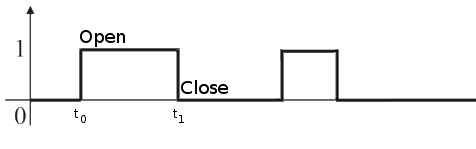
\includegraphics[scale=0.3]{gfx/graph.png}
      \caption{Sémantique des rôles}
      \label{fig:semofroles}
\end{figure}

En pratique, pour fournir cette sémantique temporelle à l'application, l'implémentation d'un rôle doit être filtrée pour isoler les séquences de donnée atypiques (bruit). Par exemple, pour un rôle joué par un capteur de contact, s'il fournit deux valeurs true (ouverture) consécutives, nous filtrons la seconde.

\section{Modèle d'infrastructure}
Les capteurs installés dans un domicile constituent une infrastructure qui supporte les rôles requis par les applications déployées. 
La bonne implémentation des rôles est critique quant à la fiabilité de la sensibilité au contexte de cette infrastructure. 
Cette fiabilité va au-delà des tests unitaires de chaque rôle.

Pour adresser la fiabilité de l'infrastructure, nous proposons de construire un modèle de cette infrastructure qui peut être vérifié. Ce modèle ne prend pas uniquement en compte les rôles individuels, mais également leur conformité par rapport à des règles globales en rapport avec l'infrastructure de capteurs.


\subsection{Les évènements de rôle}\label{archi:algebra} 
La première étape pour expliciter le modèle d'infrastructure en tant qu'ensemble de règle, est de délimiter le domaine des objets sur lesquels les règles pourront agir: les évènements de rôle. Un rôle se compose de trois éléments: (1) une interaction qui s'est produite (2) à une localisation donnée, (3) pendant une période de temps spécifique. Tout d'abord examinons la notion de période. Elle est définie en tant qu'intervalle délimitée par deux horodatage. Tel que, \begin{displaymath}\label{archi:algebra:period1}
 \begin{array}{c} 
  Period = \mathds{N}^2\\
    For~p \in Period, p = <t_1, t_2>~and~t_1~<~t_2
 \end{array}
\end{displaymath}

Une période peut également être vue comme une valeur de temps, de $t_1$ à $t_2$, croissante, qui incrémente d'une seconde -- une granularité plus fine n'est pas nécessaire en pratique. Nous pouvons alors utiliser les opérations basiques sur les ensembles pour opérer les périodes, comme $\subseteq, \supseteq$.

Enfin, un évènement de rôle est une interaction qui est arrivée pendant une période. L'ensemble d'interactions est définie par $Inter$ ({\em e.g.,} Présence, Ouverture, Utilisation). Un ensemble de localisations, $Loc$, spécifie l'emplacement d'intérêt dans le domicile ({\em e.g.,} Cuisine, Salle de bain, Chambre). Les évènements de rôle sont donc définies comme suit.

\begin{displaymath}\label{archi:algebra:event}
  \begin{array}{c}
    e~\in~Event = Inter \times Loc \times Period \\
  \end{array}
\end{displaymath}

Comme l'infrastructure de capteurs surveille le domicile, elle produite des logs de données structurés en flux d'évènements de rôles, définie précédemment. Le log d'évènements de rôles est définie ainsi $log~\in~Log = \mathscr{P}(Event)$

\subsection{Formuler des règles}
Maintenant que les logs d'évènements de rôles sont définies et peuvent ainsi être manipulés, nous nous intéressons aux règles du modèle d'infrastructure. Ces règles sont exprimées en tant qu'ensemble de formules logiques dans le calcul de prédicats du premier ordre. Nous introduisons ces règles en examinant trois exemples de notre cas d'utilisation.

\myparagraph{Présence dans la cuisine.} Cette règle rend explicite la dépendance des capteurs dans la cuisine. En substance, nous voulons exprimer le fait que chaque interaction détectée, qui n'est pas un mouvement, doit être encadré par une interaction de mouvement. Ce faisant, nous exprimons le fait que le capteur de mouvement dans la cuisine entoure toutes les autres interactions dans la cuisine ({\em e.g.,} porte de placard, machine à café). Une fois exprimée, cette sémantique assure la conformité des relevés de capteurs dans la cuisine.

Notre règle de présence dans la cuisine prend un évènement de rôle situé dans la cuisine et un log; définie ainsi. \begin{displaymath}\label{archi:algebra:example}
  \begin{array}{c}
    \forall~<i, Kitchen, p>~\in~Log, i \neq Presence~ \Rightarrow \\
    ~~~~\exists~ <Presence, Kitchen, p'>~\in~Log,~p \subseteq p' 
  \end{array}
\end{displaymath}

\myparagraph{Portes restées ouverte.} Nous supposons que dans un but d'assistance domiciliaire, une porte équipée d'un capteur de contact ne doit pas resté ouvert au-delà d'une certaine période, notée $MAX$. Une telle règle s'applique typiquement sur la porte du frigidaire et sur la porte d'entrée parce qu'elle ne doivent pas restées ouvertes trop longtemps. La durée $MAX$ peut variée en fonction des préférences de l'utilisateur et du type de porte.

Cette règle prend un évènement de rôle d'ouverture et une log; définie ainsi.
\begin{displaymath}\label{archi:algebra:example2}
  \begin{array}{c}
    \forall~<Opening, l, p>~\in~Log \Rightarrow  \# p < MAX
  \end{array}
\end{displaymath}

Notons qu'une porte restée ouverte peut être associée à un dysfonctionnement du capteur, ou bien l'utilisateur a tout simplement oublié cette porte et celle-ci n'est pas surveillée par une application déclanchant une notification de sécurité. Par exemple, la porte du placard de notre cas d'utilisation est surveillée pour rappeler à l'utilisateur de préparer ses repas, non pas pour lui rappeler qu'elle est restée ouverte.

\myparagraph{Non omniprésence.}Certaine règle de conformité peuvent être spécifiques à la localisation d'action de l'application. Par exemple, nos recherches en informatique ubiquitaire est principalement concentrée sur le maintien à domicile de personnes âgées vivant seule. Cette situation nous permet de définir la règle de conformité suivante: un rôle de présence ne peut pas être détecté simultanément à deux emplacements différents. La règle de non onmiprésence est définie ainsi. 
\begin{displaymath}\label{archi:algebra:example3}
  \begin{array}{c}
    \forall~<Presence, l, p>~\in~Log \Rightarrow \\
     ~~~~\nexists~ <Presence, l', p'>~\in~Log,~l \neq l' \wedge ~p' \cap p \neq \emptyset
  \end{array}
\end{displaymath}

En pratique, définir des règles de conformités fournis des instructions détaillées pour installer et positionner les capteurs dans le monde physique. Par exemple, la règle de présence dans la cuisine nécessite que la présence soit reconnue dans la cuisine entière. Une fois un domicile installé, les règles assurent la conformité entre l'installation et le modèle.
%\section{Architecture}
\section{Validation}



Premièrement, nous présentons succinctement l'architecture et son implémentation pour vérifier en continue qu'une installation est conforme à son modèle. Ensuite nous présentons brièvement l'expérimentation que nous avons utilisé pour collecter des données de logs écologiques. Nous définissons ensuite les règles de conformité pour un modèle de rôle dédié à l'assistance domiciliaire pour personnes âgées. Finalement, nous appliquons ces règles sur les logs pour assurer leur capacité à détecter les violations de conformité.

\subsection{Architecture}
Globalement, notre architecture consiste à abstraire les lectures brutes de catpeurs à travers une couche de rôles, alimentant à la fois les applications avec des valeurs haut niveau, et les logs d'évènements de rôles utilisés par les règles de conformité du modèle d'infrastructure. Cette architecture est décrite en Figure~\ref{fig:archi}.

Les évènements de rôles sont traités simultanément par les applications et le composant de logs. Ce faisant, la conformité des règles peut etre executée à la volée pour relever les érreurs quand elles apparaissent. Alternativement, les règles peuvent être exécutées hors ligne pour diagnostiquer des problèmes quand un opérateur est disponible pour de la maintenance.

\begin{figure}[!h]
  %\vspace{-0.2cm}
  \centering
  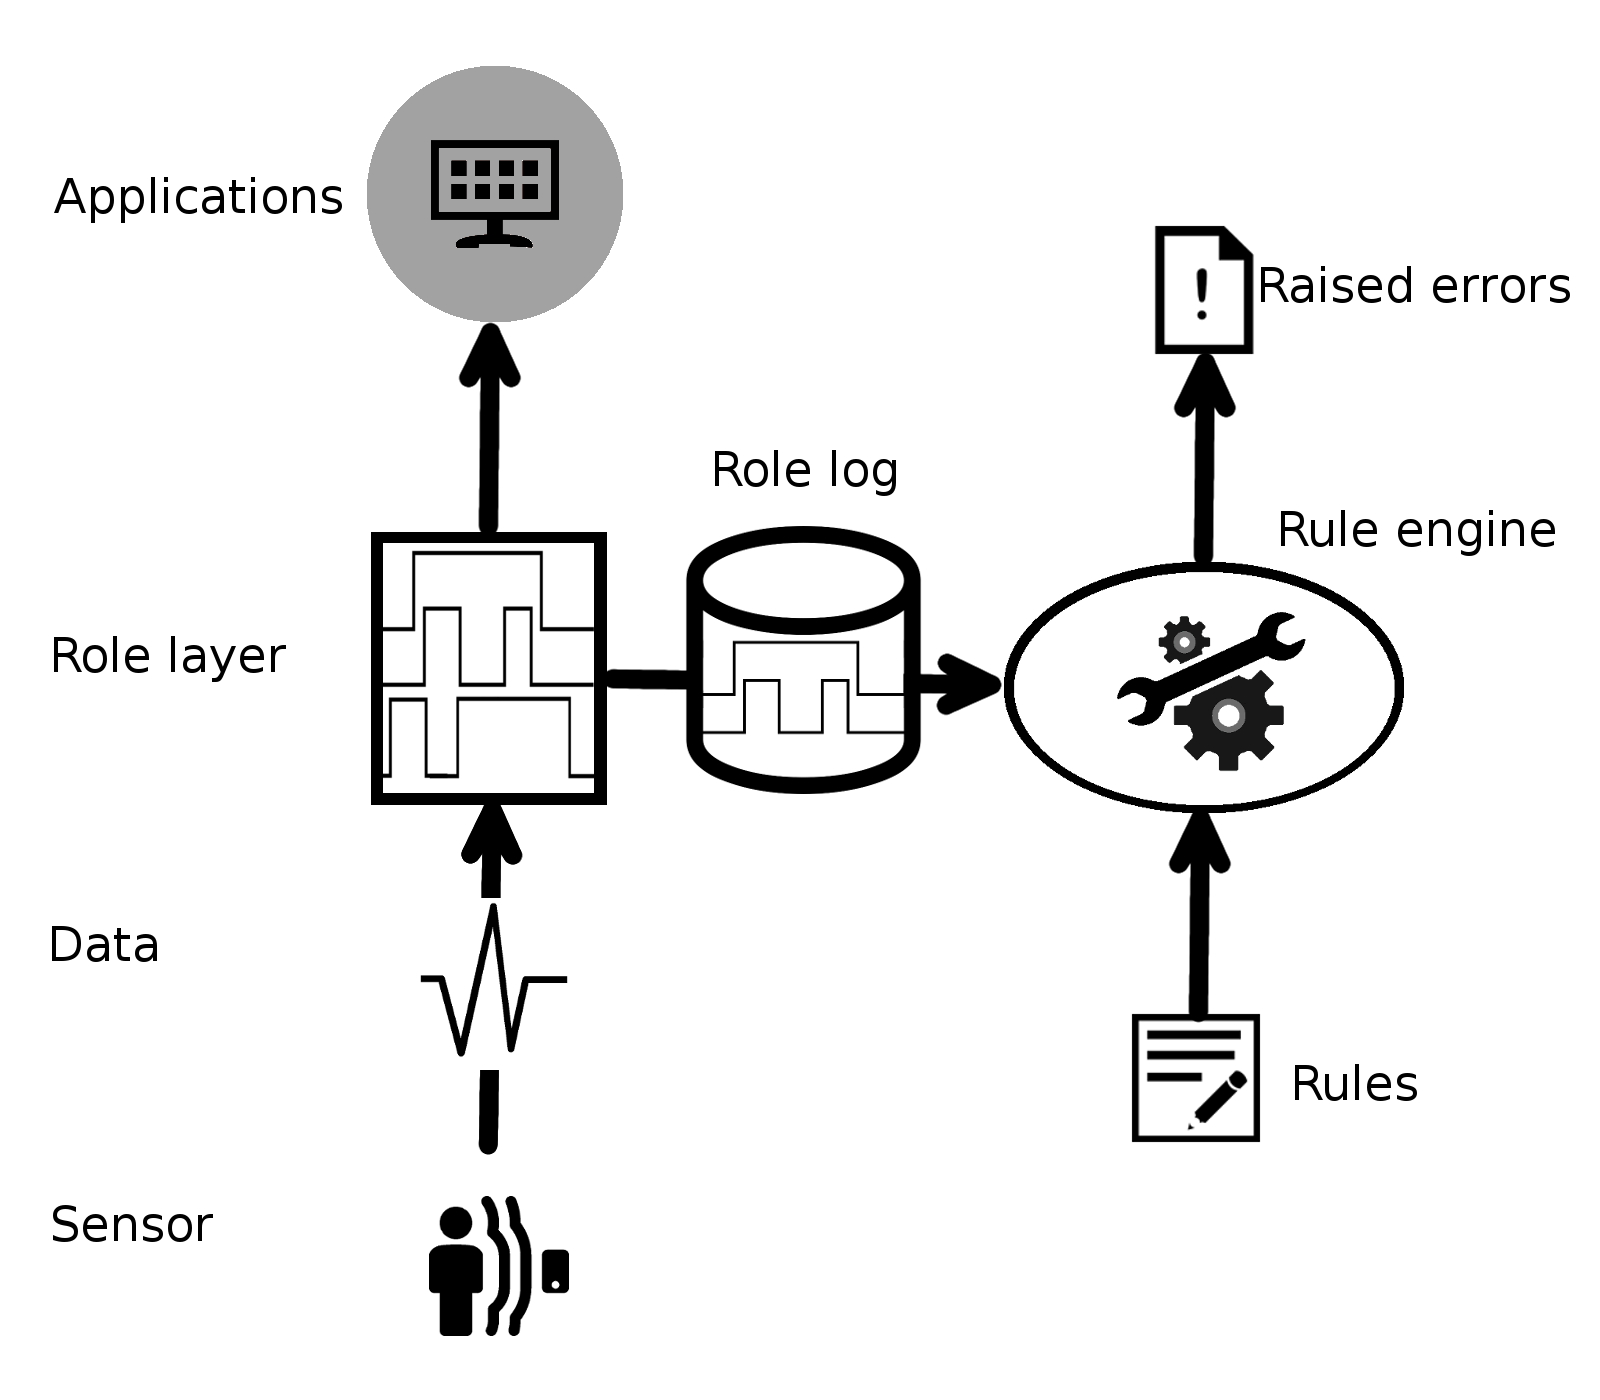
\includegraphics[scale=0.15]{gfx/architecture.png}
  \caption{Architecture}
  \label{fig:archi}
\end{figure}

Au-delà de la maintenance, les logs d'évènements de rôle peuvent aussi être précieux à des fins d'analyse sur l'évolution des activité quotidiennes des personnes âgées. En effet, ces logs permettent des analyses longitudinales qui peuvent, le cas échéant, révéler des dégradation cognitives dues au vieillissement. Ces analyse permettent au professionnel d'adapter l'assistance en supprimant ou installant de nouvelles application pour satisfaire l'évolution des besoins des utilisateurs. 

Également, en faisant levier sur les logs d'évènements de rôle, la reconnaissance d'activités du quotidien peut être ajustée. Par exemple, le seuil de déclanchement des notifications peut être modifié pour prévenir la fatigue de l'utilisateur. De plus, ces logs peuvent servir pour rejouer des séquences d'interactions et déboguer des applications au comportement erroné.


%\subsection{Implementation}\label{algebra:impl}
%This section focuses on the components needed to implement the conformance rules. Our implementation revolves around Prolog because it allows to naturally express our rules and efficiently performs conformance checking.

\myparagraph{Règles.}
Les règles de conformité sont implémenté en tant que prédicats Prolog, de même pour les opérateurs manipulant les évènements de rôles. 
%More precisely, {\em inter\_e/2}, {\em locat\_e/2}, and {\em period\_e/2} allow to access the interaction, the location, and the period of an event, respectively, or to check their equality to a given constant. Operator {\em subset\_e/2} checks whether the period of an event is included in the period of another event.

\myparagraph{Analyser de rôles.}
La plate-forme d'assistance utilisée pour valider notre approche ne fournissant pas la couche d'abstractions nécessaire pour produire les rôle, nous simulons cette couche dans notre implémentation de cette architecture en utilisant un ``analyseur de rôles''. Ce composant construit un log d'évènements de rôles en transformant le log de lecture de capteurs les informations associées (type de capteur, localisation, état et horodatage). Cet analyseur de rôle est implanté en un module C++.

\myparagraph{Moteur de règle.}
Ce module traite le log d'évènement de rôle produit par l'analyseur de rôles, et appelle un interpréteur Prolog pour executer chaque règles. De cette façon, quand une règle échoue, le moteur de règle identifie les évènements de rôle impliqué et produit une liste d'évènements de rôles non conformes avec les règles qu'ils ont fait échoués. Ce module est également implanté en C++. 

\subsection{L'expérimentation DomAssist}\label{validation:domassist}
Le projet DomAssist\footnote{ \tiny http://phoenix.inria.fr/research-projects/homeassist} vise à prolonger la vie en indépendance de personnes âgées dans leur propre domicile en leur fournissant une plate-forme d'assistance domiciliaire avec des applications aidant dans les activités du quotidien. Des egrothératpeutes, psychologues et experts en vieillissement ont définie quelles activités sont doivent être surveillées et l'ensemble d'interactions avec l'environnement qui doivent être mesurées.

Pour ce projet, deux types d'applications ont été définit: (1) des application pour surveiller les activités du quotidien et assister l'utilisateur quand elle n'ont pas été effectuée, et (2) des applications de sécurité pour sécuriser le domicile ({\em e.g.,} porte d'entrée restée ouverte). Une étude utilisateur a été conduite en recrutant 24 participants et en déployant à leur domicile notre plate-forme d'assistance domiciliaire pour une durée de neuf mois. Nous avons utilisé les données collectées durant le projet DomAssist pour valider notre modèle d'infrastructure.

\subsection{Modèle}\label{validation:model} 

Les capteurs utilisés dans DomAssist Permettent de mesurer douze points d'interactions avec l'environnement. Les interactions de présence sont mesurées avec des capteurs de mouvement, les ouvertures sont mesurées avec des capteurs de contact, et l'utilisation des appareils électriques est mesurée avec des capteurs de consommation électrique. La configuration de DomAssist en terme de capteurs et leur rôles associés est résumé dans le tableau~\ref{tab:domassist:role}.

\begin{table}[h!]
  \centering
  \begin{tabular}{|l|l|l|}
    \hline
    Room & Role & Sensor \\
    \hline
    \multirow{5}{*}{Kitchen} & Coffee maker in use & EM \\
    & Cabinet door open & CS \\
    & Fridge door open & CS \\
    & Microwave in use & EM \\
    & Presence & CS \\
    \hline
    \multirow{2}{*}{Entrance} & Door open & CS \\
    & Presence & MD \\
    \hline
    \multirow{2}{*}{Bathroom} & Shower in use & MD \\
    & Presence & MD \\
    \hline
    \multirow{2}{*}{Bedroom} & Dressing open & CS \\
    & Bedside lamp in use & EM \\
    & Presence & MD\\
    \hline
  \end{tabular}
\ \\ EM = Electric Meter, CS = Contact Sensor,\\ MD = Motion Detector.
  \caption{Rôles dans DomAssist}
  \label{tab:domassist:role}
\end{table}

Pour des raisons pratiques, notre approche n'a pas été déployée au démarrage du projet DomAssist. Au lieu de quoi, nous avons appliqué notre approche a posteriori. Notre modèle a donc été utilisé rétrospectivement pour vérifier la conformité du domicile de chaque participant en exécutant les règles sur les logs accumulés durant l'expérimentation.

En étudiant l'expérimentation et nos rôles, nous avons spécifié les règles de conformité qui rendent explicite les paramètres de l'étude. C'est à dire, les participants vivent seul (règle de non omniprésence) et des interactions avec l'environnement qui doivent suivre un motif spécifique (porte restée ouverte). D'autres règles ne dépendent pas du but de l'étude et peuvent être généralisées. La règle d'inclusion de présence et ses raffinements (intersection de présence et besoin de présence) en sont des illustrations.

Examinons maintenant ces règles.

\myparagraph{Non omniprésence.}
Rappelons que cette règle assure qu'un rôle de présence n'est pas détecté simultanément à deux localisations différentes. En pratique, en fonction de la réactivité des capteurs de mouvements utilisés pour implémenté la détection de présence, quelques chevauchements peuvent survenir et doivent être ignorés. Typiquement, un détecteur de présence signale une absence avec une latence, permettant à l'utilisateur d'être détecté dans une autre pièce. Il peut donc arrivé que la présence soit détectée simultanément dans deux endroits différents pendant un court instant.


% Remove the following rule, as it may be too easily violated by users missing an activity
%\paragraph{Trigger rates}
%We assume that an interaction has to be performed at least once each 24 hours. This element of the model is border closed to activity recognition. A role that has not been recognized for a critical time may be the result of a breach of activity achievement from the user, or a failure from sensors used to measure the interaction. Nevertheless, it is the aim of the activity recognition application to raise user fail. Consequently, in the context of {\HomeAssist} installation, this rule is used to raise failure regardless of user failure.

\myparagraph{Porte restée ouverte.}
Cette règle assure que la période d'un rôle d'ouverte ne dure pas plus d'un certain temps (trois heures dans notre configuration). Notons que cette rèlge est exécutée sur les logs d'évènements de rôle et ne prend pas en compte la façon dont les applications d'assistance peuvent réagir à une telle situation. Par exemple, DomAssist contient une application qui surveille la porte d'entrée et notifie l'utilisateur quand la porte est restée ouverte et sans surveillance, pour quelques minutes (la durée est configurée en fonction du l'utilisateur). En pratique, quand elle est appliquée aux logs de notre études, cette règle détecte dans la plupart des cas des problèmes d'installation. Une des raisons est que les participants sont routinisés dans leur activités~\cite{BERGUA-RESTRICTION-IJAHD2013} et n'ont pas décliné congnitivement de façon significative durant l'étude.

\myparagraph{Inclusion de présence.}
Chaque pièce pour laquelle une interaction doit être détectée est équipé avec un détecteur de mouvement. Par concéquent, nous avons généralisé la règle de présence dans la cuisine comme suit: toute interaction a une localisation donnée, qui n'est pas une présence, doit être inclue dans un rôle de présence à la même localisation. 

% In practice, this rule may fail to apply to a specific location: the entrance. Indeed, when users comes back home, they first open the entrance door, then come inside the home to be detected by the motion sensor. Thus, the Door opening role event cannot be surrounded by the Presence role event because the latter one is measured inside the home.  To resolve this problem, the Presence inclusion rule is not applied to the roles related to the entrance. To refine the diagnostic of the Presence inclusion rule, we introduce next two rules towards identifying the cause of the violation.

\myparagraph{Intersection de présence.}
L'inclusion de présence peut être trop contraignante pour s'appliquer à certaines situations. Parfois, nous devons simplement nous assurer que la présence et d'autres interactions ont une intersections non-nulle quand elle sont située dans la même pièce. Une telle règle s'applique dans l'entrée du domicile, équipée d'un capteur de contact sur la porte d'entrée et un capteur de mouvement pour la zone de l'entrée. En effet, si l'utilisateur ouvre la porte depuis l'extérieur ou l'intérieur, les rôles de présence et d'ouverture ont une période de temps durant laquelle leur intersection est non-nulle.


% Every role event, which is not Presence, must have a non-empty intersection with a Presence role event at the same location. If this rule is also violated, it might be the case that the presence detector is not placed correctly with respect to the non-presence interaction. Alternatively, the presence detector might be completely obstructed. To help distinguishing between these two situations, we defined the following even more lenient rule.

\myparagraph{Besoin de présence.}
Pour s'assurer que le détecteur de mouvement est toujours actif même si il est mal positionné, nous introduisons la règle suivante: chaque rôle, qui n'est pas une présence, doit être accompagné d'un évènement de rôle présence à la même localisation. Cette présence doit arriver au même moment plus ou moins dix minutes. Cette règle rend explicite le fait que le capteur de mouvement est toujours couplé avec un ou plusieurs autres capteurs dans notre configuration. La violation de cette règle indique principalement que le capteur de mouvement ne fonctionne pas correctement, il est toujours enregistré dans le système, mais n'émet plus aucune donnée.

% In theory, the misbehavior could also be due to a false positive in the non-presence interaction. However, this situation never occurred in our experiment.

\subsection{Méthodologie}\label{validation:methodology}
Nous avons collecté les logs de données des habitations de 24 participants, âgés de 80 en moyenne et habitants seuls. Les données collectées couvrent une période de neuf mois. Cependant, des problèmes techniques ({\em e.g.,} Accès internet, passerelle de capteurs, serveur) nous ont poussé à ignorer certaines périodes de temps; ces problèmes peuvent être directement détectés au niveau de la plate-forme. Les logs de DomAssist ont également été nettoyés en éliminant les évènements de rôle non conformes. Ces derniers peuvent être détectés par un simple système de surveillance de heartbeat.
% Indeed, every sensor emits a heartbeat signal, whose absence is automatically detected by the lower layers of the platform and signalled as a sensor failure.

Nous avons le plan de chaque domicile des participant ainsi que le positionnement des capteurs. Cette information est utilisée pour diagnostiquer les problèmes quand des violations de conformités arrivent dans les logs. D'autres ressources utilisées pour diagnostiquer les violations ont été utilisées comme les fichiers de suivis des interventions remplis par les professionnels chargés de faire passer des questionnaires à chaque participants durant la durée de l'étude.


\subsection{Résultats expérimentaux}\label{validation:results}


%Our goal in pruning the logs of HomeAssist was to show that our approach could detect anomalies, beyond what simple fault tolerant mechanisms could do. 

Le modèle définit pour DomAssist permet de lever deux types d'anomalies: 1) {\em les non-conformités permanentes} réfèrent à une règle systématiquement transgressée, indiquant des non-concordances permanentes entre l'infrastructure et le modèle; 2) {\em les non-conformités émergentes} correspondent a une règle qui est vérifié la plupart du temps, mais échoue occasionnellement. Examinons quelques instances de ces anomalies.

\myparagraph{Non-conformités permanentes}
Dans un domicile, l'interaction d'ouverture est détectée pour la porte de placard de la cuisine mais les règles inclusion de présence et intersection de présence échouent systématiquement. Cependant, la règle de besoin de présence n'échoue jamais, indiquant que la porte de placard est ouverte mais jamais entourée par une interaction  de présence dans la cuisine; la présence est détectée à des moments sans rapport. La consultation des documents relatifs à cette installation ont montré que ce placard n'est pas localisé dans la cuisine mais dans une pièce attenante, comme montré en Figure~\ref{fig:map}. Cette situation montre un problème dans la définition du modèle pour cette installation. En conséquence, nous avons réparé le modèle de cette installation en y supprimant les règles inclusion de présence et intersection de présence.

Dans ce même domicile, un autre problème à été identifié: la règle inclusion de présence échoue systématiquement sur le rôle d'ouverture du frigidaire, mais l'intersection de présence n'échoue jamais. Même si le frigidaire est localisé dans la cuisine, le capteur de mouvement utilisé pour mesuré la présence dans la cuisine, n'a pas été positionné pour couvrir l'ensemble de la cuisine, comme montré en Figure~\ref{fig:map}. Ce problème provient dans ce cas d'une erreur à l'installation et sa réparation requière simplement de changer le positionnement du capteur de mouvement. %However, because we retrofitted HomeAssist in our work, this operation could not be done.

Nous avons observé la même situation dans deux autres domiciles pour lesquels le placard de la cuisine équipé d'un capteur de contact est en fait situé en dehors de la cuisine.

Généralement, ces problèmes surviennent quand la plate-forme d'assistance est déployée à large échelle. Dans ce contexte, les installations sont faites par un professionnel et non par les chercheurs qui ont conçu la plate-forme et donc possèdent un savoir implicite sur la bonne manière de déployer. Dans notre cas, même pour 24 domiciles, quelques installations ont été faites par des membres n'ayant pas ce savoir et ont manqué certaines règles implicite.

\begin{figure}[!h]
  %\vspace{-0.2cm}
  \centering
      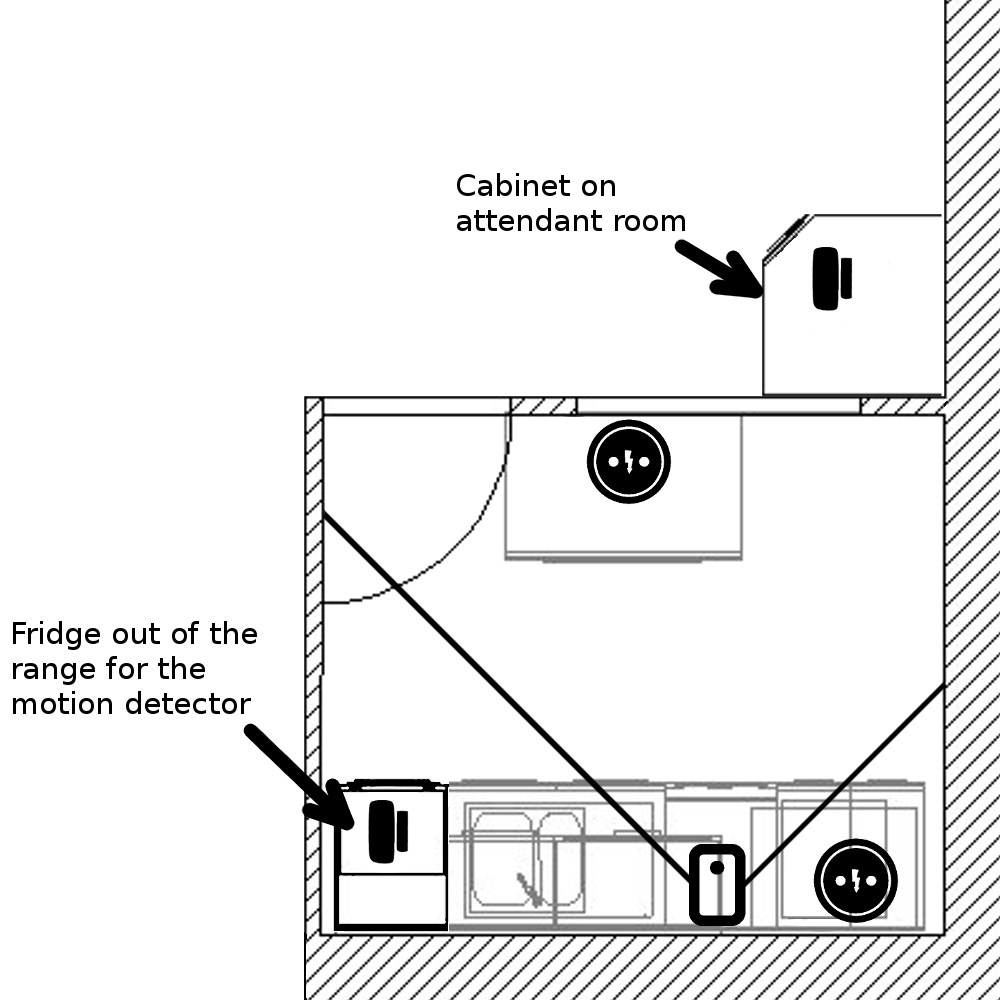
\includegraphics[scale=0.2]{gfx/map.png}
      \caption{Installation issues}
      \label{fig:map}
\end{figure}

Si notre outil avait été utilisé dès la phase de déploiement, il aurait été possible de détecter les anomalies d'installation dès le départ, pendant l'installation ou dans les premiers jours d'exploitation. Parallèlement, une fois déployés, des règles supplémentaires peuvent affiner les modèle pour prendre en compte des spécifications imprévues ({\em e.g.,} cuisine en forme de L). Une fois l'installation ou le modèle réparé, le modèle aide à la détection d'anomalies qui ne sont pas arrivées au moment de l'installation, mais après une période de fonctionnement normal.

\myparagraph{Non-conformités émergentes.}
Un motif de non-concordance a été observé dans cinq domiciles à différentes périodes de temps. Pendant plusieurs jours, la règle inclusion de présence à été enfreinte par une absence de présence dans la cuisine causée par un capteur de mouvement qui dysfonctionne. Dans chacun des cas, les règles d'intersection et de besoin de présence étaient également transgressée durant ces périodes. Cette dernière règle montre qu'aucun rôle de présence n'a été reconnu durant les 20 minutes entourant cette violation. Les résultats de ces règles fournissent de précieuses informations pour trouver la cause des dysfonctionnement relevés. Il est alors raisonnable de supposer que la cause de cet échec de la règles et un dysfonctionnement temporaire du rôle de présence. Cela suppose que le capteur de mouvement a put être obstrué ou mal orienté. 

Une situation similaire est arrivé dans l'entrée de deux autres domicile: la porte était ouverte mais aucune présence n'a été détectée.

La porte restée ouverte a été observé dans quatre domiciles à différents endroits comme le frigidaire, le placard de la cuisine ou la penderie ({\em i.e.,} la porte est restée ouverte plus de trois heures). D'après les fichiers de suivi des interventions de DomAssist, les utilisateurs concernés ont été questionnés après quelques jours sur les comportements erronés des applications reposant sur ces interactions. Ils ont indiqué que les capteurs de contact étaient tombé. Les installations ont alors été réparée par les techniciens chargés des interventions. Notre modèle, si il avait été disponible durant cette expérimentation aurait permis de rapporter ces incidents, et de les réparer plus rapidement. Cette réactivité est une clé pour les application sensibles au contexte. Elle fait la différence entre une application utile, et une application qui harcèle l'utilisateur avec des notification non pertinente.

\section{Discussion}\label{sec:discussion}
Un modèle explicite d'une infrastructure est capable de détecter les dysfonctionnements du systèmes durant la phase d'installation ou pendant l'exploitation normale. Comme suggéré par certains de nos exemples, une fois une erreur détectée, quelques techniques de diagnostique peuvent être utilisés pour identifier les rôles qui sont la source de l'erreur.  

Premièrement, si plusieurs règles sont violées en même temps, et que ces règles concernent des ensembles de capteurs qui se chevauchent, il est alors probable que le rôle à la source de cette erreur soit à rechercher à l'intersection de ces ensembles. Par exemple, quand la règle intersection de présence échoue en même temps pour le rôle présence dans la cuisine et pour différentes interactions qui ne sont pas des présences (frigidaire, placard, {\em etc.}), on peut en déduire avec une forte probabilité que le rôle défaillant est la présence dans la cuisine. 

Deuxièmement, concevoir une version raffinée d'une règle qui vérifie un ensemble de capteurs ou est un sous-ensemble de la règle de base, peut s'avérer utile pour diriger la recherche d'un rôle défaillant ou d'un capteur qui dysfonctionne. Cette idée est illustrée dans notre modèle pour DomAssist. Il y a une chaîne de trois règles $R_i$ avec des conditions de plus en plus relâchées: inclusion de présence, intersection de présence et besoin de présence. Toutes ces règles sont du type $p \rightarrow q_i$ pour $(i=1..3)$ où le postulat $p$ est identique mais la conclusion $q_i$ est de plus en plus faible. Il y a une implication tout au long de la chaîne, $R_1 \rightarrow R_2 \rightarrow R_3$, ou inversement, quand une des règles échoue, les règles les plus fortes échouent également. Basé sur l'analyse des règles, on peut définir un arbre de décision comme celui en Figure~\ref{fig:bdd} pour aider au diagnostique.

%Secondly, designing refined versions of a given rule that check a set of sensors or subsets of it, may be useful to direct the search of the failing role or malfunctioning sensor. This idea is illustrated in our model for HomeAssist. There is a chain of three rules $R_i$ that increasing relax conditions: presence inclusion, presence intersection, and presence requirement. All these rule are of the type $p \rightarrow q_i$ for $(i=1..3)$ where the premise $p$ is identical but the conclusion $q_i$ is increasingly weaker. Thus, there is an implication relation along the chain, $R_1 \rightarrow R_2 \rightarrow R_3$, or conversely, when one of the rules fails, stronger rules also do. Based on rule analysis, one can derive a binary decision tree such as the one in Figure~\ref{fig:bdd} for helping the diagnosis.

\begin{figure}[!h]
  %\vspace{-0.2cm}
  \centering
      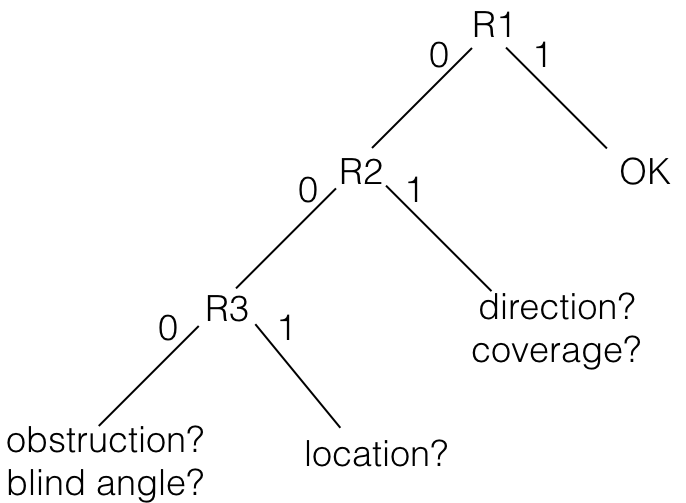
\includegraphics[scale=0.3]{gfx/bdd.png}
      \caption{Binary decision tree for helping the diagnosis}
      \label{fig:bdd}
\end{figure}



%When studying some of the systematic mismatches between the installation and a correct model, one may legitimately ask: How come these installation issues were undetected by conventional tests at installation time? For instance, the fridge or cabinets placed outside the kitchen would have necessarily failed any test of the breakfast monitoring application. This argument is valid: all {\em installed} applications were indeed tested in every home at installation time. However, the experimental protocol allowed participants to choose which applications to activate, based on their needs and preferences. As a result, the breakfast monitoring application was not installed in several homes, hence the undetected installation anomalies. If our model had been used at installation time, the installations could have been certified as conform to the model, validating all applications based on this model.

L'utilité de notre approche pour s'assurer continuellement la conformité d'une infrastructure va au-delà de notre étude. Premièrement, un modèle d'infratrustructure fourni un modèle de référence pour les des applications disponibles dans un catalogue en ligne, comme un Appstore: une application peut être installée du moment qu'elle est conforme au modèle d'infrastructure. Deuxièmement, vérifier le modèle au moment de l'installation réduit les besoins de tests pour {\em toutes} les applications déployées pour une installations donnée, pourvu que le modèle couvre toutes les hypothèses requises par les applications.

\section{Conclusion}\label{sec:futurework}
Nous avons montré que les applications sensibles au contexte produisent fréquemment des suppositions implicites sur l'infrastructure de capteurs. Ces suppositions sont typiquement traduites en déclarations conditionnelles qui polluent le code avec des préoccupations non fonctionnelles. Cette approche défensive peut être évitée en exprimant ces suppositions, non pas dans le code des applications, mais en les factorisant en un modèle explicite d'infrastructure de capteurs. Non seulement la violation d'une telle règle permet d'alerter rapidement sur un dysfonctionnement de l'installation, mais contribue également à diagnostiquer le problème. Une telle approche permet non seulement de s'assurer de la fiabilité de la sensibilité au contexte des applications d'assistance domiciliaire, mais également la définition du modèle, permet de de fournir des instructions détaillée quant à l'installations des capteurs dans le domicile, randant ce dernier sensible au contexte.



% Our approach has been implemented in the context of an assisted living platform, running a set of applications dedicated to assist senior users. Our tool was applied to real sensor data collected during a 9-month field study, consisting of 24 participants aged 80 on average. The results show that some latent installation mistakes could have been found at installation time, using our model. Furthermore, several sensor problems that occurred during operation could have been detected on the fly and repaired more promptly to ensure the reliability of context-awareness applications.

% In future work, we will apply our method in a larger deployment consisting in hundreds of installations. This setting will allow us to quantify in more detail the improved reactivity in detecting emerging infrastructure issues, remotely diagnosing the underlying failure, and repairing the platform on-site. Another future work will consist of proposing log visualisation techniques and tools that contribute to identify new rules for the model by recognizing regular event patterns and anomalies. 
\chapter{Unifier la définition de services sensibles au contexte}
\begin{preamble}
Dans ce chapitre nous analysons un large éventail de services d'assistance domiciliaire dédié aux personnes âgées, en considérant la variété des besoins des intervenants, pour identifier les concepts clés et les opérations spécifiques pour le traitement de la sensibilité au contexte. Reposant sur cette analyse, nous proposons un langage dédié et sensible au contexte avec son architecture logicielle. Cette approche permet de mettre en synergie les intervenants d'une maison sensible au contexte, en leur fournissant une approche unifiée pour concevoir et développer des services.
\end{preamble}
\chpsummary{Contributions}
{
{\em Analyse de domain} Identification des concepts clés et des opérations spécifiques au traitement sensible au contexte.;
{\em Langage dédié} Un langage spécifique pour développer un large spectre de services sensibles au contexte, avec un haut niveau d'asbtraction et un traitement uniforme de source de données hétérogènes.;
%\myparagraph{Compiler} We have implemented a compiler for our DSL that maps high-level rules into low-level requests, crunched by an event-processing engine.
{\em Validation} re-définition de 55 services, couvrant les besoins de tous les intervenants d'une plate-forme d'assistance pour le maintien à domicile de personnes âgées.
}


La notion de {\em contexte} est fondamentales dans les champ de l'informatique ubiquitaire et englobe de beaucoup de dimensions, le monde physique, un individu, ses activités, les technologies déployées, etc~\cite{bauer2012comparison}.
% This wide range of dimensions is reflected in the host of application areas that leverages context awareness, spanning infrastructures ({\em e.g.,} railways), premises ({\em e.g.,} buildings), and health ({\em e.g.,} physiological status). 
Une attention particulière de la recherche a été portée sur le {\em domicile} ({\em e.g.,}~\cite{cook2013casas,feminella2014piloteur}). Ce périmètre implique beaucoup de dimensions contextuelles, notamment les interactions physiques avec l'environnement ({\em i.e.,} capteurs), les interactions numériques avec l'environnement de l'utilisateur ({\em i.e.,} email, agenda), l'état des nombreux composants de l'infrastructure de l'informatique ubiquitaire (matériel, logiciel et réseau), les préoccupations relatives aux applications ({\em i.e.,} détection d'activité). Concernant la population générale, le défit récurant est d;identifier de quels services ont besoins les utilisateurs~\cite{brush2011home}, et plus généralement, de développer de méthodes pour recueillir et analyser ces besoins~\cite{coutaz2010disqo}.

Toutefois, dans le domaine du maintien à domicile de personne âgées, un tel environnement peut fournir
des services d’assistance pour pallier les pertes cognitives dues au vieillissement et assurer une vie
indépendante({\em e.g.,} ~\cite{rashidi2013survey}). Ces services sont principalement: (1) détecter et rappeler les activités du quotidien ({\em e.g.,} préparation de repas, toilette, se coucher) pour maintenir le status fonctionnel de l'utilisateur~\cite{caroux2014verification} et (2) surveiller les situations potentiellement dangereuses ({\em e.g.,} cuisinière, porte d'entrée) pour garantir la sécurité de l'utilisateur~\cite{rashidi2013survey}. 
Parce qu’elle implique plusieurs disciplines, une maison équipée d’informatique ubiquitaire et
dédiée au maintien à domicile de personnes âgées demande l’implication d’une variété d’intervenants, tant pour concevoir et développer des services d’assistance, que pour déployer et maintenir l’infrastructure sous-jacente. De ce fait parmi ces intervenants on retrouve les personnes âgées elle-même, les aidants, les expets en vieillissement, les professionnels de santé, les développeurs d'applications ainsi que les techniciens de maintenance. 
Cette grande diversité d’intervenants correspond à une diversité
de contextes : les services de chaque intervenant repose sur des contextes spécifiques (état des
capteurs pour la maintenance, utilisation du frigidaire pour l’assistance à domicile). Ces différents
contextes sont généralement étudiés séparément, en silo. Typiquement, chaque intervenant développe sa propre approche, pour extraire ses informations contextuelles, empêchant toute synergie.

Nous avons analysé un large éventail de services d'assistance domiciliaire dédié aux personnes âgées, en considérant la variété des besoins des intervenants. Ces services sont installés sur une plate-forme d'assistance domiciliaire déployée chez 129 personnes âgées vivant seules et âgées de 82 ans en moyenne~\cite{consel2017homeassist}. 
Cette analyse a permis d'identifier les concepts commun et les variations
entre différentes couches de services déployés et utilisés au quotidien,
pour en extraire des concepts clés et des opérations spécifiques aux
traitements sensibles au contexte.

%\subsection*{Our Approach}

Nous basant sur cette analyse, nous proposons un langage de spécifique, sensible au contexte, appelé Maloya et son architecture logiciel, qui fournie un cadre de conception et les outils pour concevoir et développer des services domiciliaires. Pour unifier les source hétérogènes de données, de composants matériels aux composant logiciels, notre approche promeut un paradigme ``centré données'' et ``orienté données''. Notre approche est {\em centrée données} pour fournir une vue canonique des données mesurée à l'ensemble des services, couvrant les services de maintenance requérant l'état bas niveau des capteurs, jusqu'aux services spécifiques aux aidants nécessitants des mesures d'activités de haut niveau. Notre approche est {\em orientée données} avec des services définis en terme de règles traitant des évènements et des états.


% To unify the way services are developed, our approach introduces abstractions and notations that are specific to context-aware processing. The resulting {\em domain-specific language} (DSL) covers the needs of the stakeholders and provides an abstraction layer over underlying, well-established concepts and technologies, such as Allen's algebra to express sequences of interactions~\cite{Allen} and complex-event-processing engines to efficiently process the rules generated from DSL services ({\em e.g.,}~\cite{Cugola:2012:PFI:2187671.2187677}). Furthermore, we envision that our language can serve as a high-level stepping stone to introduce end-user programming languages for stakeholders with no computer-programming background.

% To validate our approach, we have re-implemented 55 services ranging over all the stakeholders of the assisted living platform under study. These new services were deployed and successfully tested for their effectiveness in performing the specific tasks of the stakeholders: detection of daily activities, detection of user risks, sensor failure, {\em etc.}

% \subsection*{Contributions}
% To summarize, this paper makes the following contributions.

% \myparagraph {Domain analysis} We provide an analysis of context-aware processing layers in the domain of aging in place. From this analysis, we identify key concepts and operations specific to context-aware processing.

% \myparagraph {Domain-specific language} We introduce a language, specific to developing context-aware services, providing high-level abstractions and notations. 
% Underlying this language is a data-centric and data-driven paradigm that allows services from a range of stakeholders to uniformly process heterogeneous sources of sensed data.

% \myparagraph{Compiler} We have implemented a compiler for our DSL that maps high-level rules into low-level requests, crunched by an event-processing engine.

% \myparagraph {Validation} We applied our approach to re-implement 55 services, ranging over all the stakeholders of an assisted living platform dedicated to aging in place. The resulting services are expressed at a high level and are effective in performing the tasks of the stakeholders.





\section{Analyse du domaine}
Pour vérifier s'il est possible d'unifier la conception de services sensibles au contexte dans le cadre du maintien a domicile des personnes âgées, il est indispensable d'analyser le domaine afin d'identifier, le cas échéant, les implications d'une telle approche et quels sont les éléments indispensables à prendre en compte.
Le domaine de la sensibilité au contexte dans le maintien à domicile des personnes âgées reste jeune et le chemin vers l'adoption est encore en étude~\cite{kaye2017making}. La littérature comporte encore peu d'articles concernant le déploiement de solutions d'assistances dans le domicile réel d'utilisateurs ({\em e.g.,} \cite{kaye2011intelligent}). Cependant, nous avons pu faire levier sur le projet DomAssist pour conduire notre analyse du domaine.

\subsection{DomAssist: Un domicile sensible au contexte pour le maintien à domicile des personnes âgées}

DomAssist est une plate-forme d'assistance qui fournit un catalogue d'applications d'assistance, pour le support des activités du quotidien, la sécurité de l'utilisateur et ses interactions sociales~\cite{consel2017homeassist}. DomAssist est déployée les domiciles de 129 personnes vivants seule âgées de 82 ans en moyenne, pour une durée de 12 mois.

DomAssist est un parfait cas d'étude sur lequel construire une approche unifier pour développer des services pour domiciles sensibles au contexte dédié au maintien a domicile. Il rassemble tout les besoins pour viser notre but: (1) il est déployé dans des environnements réels; (2) il supporte le maintien a domicile de personnes âgées avec des utilisateur fragiles et des besoins immédiats; (3) l'étude conduite est suffisamment longue pour que les problèmes de maintenances et d'évolution aient à être traité rigoureusement; (4) la plate-forme est déployée à une échelle suffisamment large pour que l'administration des domiciles sensibles au contexte ait besoin d'être supporté par des services; (5) les services existant reflètent un large éventail de besoins exprimés par les intervenants, couvrant les utilisateurs, les aidants, les ergothérapeutes, les psychologues, les experts en facteurs humains, les techniciens d'installation et de maintenance, et les informaticiens.

Décrivons maintenant la plate-forme pour délimiter la courverture des services sensibles au contexte. DomAssist se compose d'une architecture client-serveur, pour laquelle le serveur instancie autant de machine virtuelle qu'il y a de domicile sensible au contexte. Chaque machine virtuelle exécute les services d'assistance selectionnés par l'utilisateur et ses aidants. Ces services d'assistance sont alimentés par des données envoyées par Internet via une passerelle déployée dans le domicile. Cette passerelle rassemble les informations en provenance des capteurs placés dans des endroits stratégiques pour surveiller les activités. 
 As well, the gateway channels actions from the services to the home's actuators. In the HomeAssist field study, a typical home consists of 4 contact sensors (entrance door, drawers, cabinets, {\em etc.}), 6 motion detectors (entrance area, kitchen, bathroom, {\em etc.}), and 2 smart plugs, which measure the electricity consumption and turn on/off a connected appliance (microwave, light path, coffeemaker, {\em etc.}). The number and type of devices can vary depending on the configuration of the home and the activities to be monitored. Finally, the home is equipped with a stationary tablet, placed at a central location in the home and always connected to a power outlet. This tablet is dedicated to interacting with the user via notifications emitted by assistive applications, which need to alert the user of a given situation ({\em e.g.} unattended entrance door left open)~\cite{consel2015unifying}.

% Let us now illustrate the diversity of issues addressed by HomeAssist with a set of existing scenarios dedicated to support aging in place.




%**********************************************
\subsection{Scénarios pour le maintien à domicile}\label{domain:scenario}
Nous présentons maintenant quatre scénarios illustrant la variété d'intervenants et de préoccupations nécessaires au support du maintien à domicile de personnes âgées à l'aide d'une maison sensible au contexte (voir Figure~\ref{scenario-fig}). Le premier scénario adresse la sécurité de l'utilisateur. Ce scénario surveille la porte d'entrée pour s'assurer qu'elle ne reste pas ouverte trop longtemps sans être surveillée. Le deuxième scénario, se rapporte au besoin de l'aidant en terme de surveillance des activités du quotidien, en particulier, les routines de préparation de repas. Les deux dernier scénarios concernent des besoins exprimés par les techniciens pour garder les domiciles sensible au contexte opérationnels. Le premier scénario de maintenance détecte l'utilisation d'un placard sans que celle-ci soit recouverte par la détection d'une présence. Le second scénario de maintenance détecte quand un capteur échoue à communiquer; cette situation se produit lorsque le capteur n'a plus de batterie ou dysfonctionne.

\begin{figure*}[t]
\begin{tabular}{| l | l | l | p{7cm} |} \hline
{\bf Stakeholder} & {\bf Domain} & {\bf Name} & {\bf Description} \\ \hline \hline
Older adult& Safety & Door Alert & Entrance door \uline{is open} and  \uline{is unattended} \dotuline{for 5 minutes} \\ \hline
Caregiver & \begin{tabular}{ll} Daily \\ Activities \end{tabular} 
       & \begin{tabular}{ll} Reheating \\ A Frozen Meal\end{tabular} 
          & Freezer \dashuline{gets used} and stove \dashuline{gets turned on} \dotuline{within 10 minutes} or Freezer \dashuline{gets used} during stove \uline{is on},
during \uline{lunch time} (or dinner time) \\ \hline
\begin{tabular}{ll} Home \\Technician \end{tabular}
               & Maintenance & \begin{tabular}{ll} Presence \\ Dependency\end{tabular} 
                  & Whenever the cupboard \dashuline{gets opened} in the kitchen, a presence in the kitchen \uline{is true} \\ \hline
\begin{tabular}{ll} Home \\Technician \end{tabular}
   & Maintenance 
        & \begin{tabular}{ll} Communication \\ Failure \end{tabular} 
             & A sensor \uline{fails to communicate} \dotuline{for 24 hours} and its status does not \dashuline{get updated} \\ \hline
\end{tabular}
\caption{Example scenarios for assistive services}
\label{scenario-fig}
\end{figure*}

Ces scénario offre un apperçu sur les type de services sensibles au contexte nécessaire pour supporter le maintien à domicile de personnes âgées. Certains services tels que ``Door Alert'', peuvent convenir à la plupart des utilisateur. En revanche d'autres services, typiquement, les services concernant les activités du quotidien nécessite un certain degrée de personnalisation pour être efficace. Ceci est illustré par l'activité de préparation de repas et le scénario ``Reheating a Frozen Meal''.

De la même manière, ``Communication Failure'' peut s'appliquer à n'importe quel domicile sensible au contexte, alors que ``Presence Dependency'' demande d'instancier les règles en fonction de la localisation des capteurs. 

\subsection{Analyse de commonalités et variabilités}
Pour conduire notre analyse du domaine, nous avons examiné un éventail de services offert par DomAssist pour identifier leurs commonalités et leurs variabilités. Ces services sont développés en Java en utilisant une méthodologie de conception outillée~\cite{bertran2014diasuite,cassou2012toward}.

We now present the outcomes of this analysis that take the form of high-level, domain-specific concepts. These concepts will pave the way to our domain-specific approach presented in the next section.

\myparagraph{Commonalités} Tous les services se réfèrent à une notion d'{\em environnement} à partir duquel effectuer les mesures. Ces mesures englobent les interactions à la fois dans l'environnement physique ({\em e.g.,} un mouvement détecté) et dans l'environnement numérique ({\em e.g.,} un rappel d'évènement délivré par un agenda). De plus, nous avons identifié deux concepts complémentaires associé à l'environnement: évènements et états. D'un côté, un {\em évènement} définie une mesure d'environnement qui change ({\em e.g.,} une porte devient ouverte/fermée) -- les évènements sont soulignés avec des pointillés dans les scénarios de la Figure~\ref{scenario-fig}. D'un autre côté, un {\em état} rend un évènements persistant à travers le temps ({\em e.g.,} la porte {\em est} ouverte) -- les états sous soulignés avec une ligne pleine dans la Figure~\ref{scenario-fig}. Une fois ces concepts identifiés, nous définissons les façons spécifiques de les combiner, exposant les commonalités de {\em composition}. Spécifiquement, la combinaison de mesures d'environnement peut définir un {\em ordre} dans lequel les interaction doivent arriver et leur {\em durée} -- ces contraintes sont soulignées avec des points dans la Figure~\ref{scenario-fig}.

Étudions plus en détail ces points communs en examinant leur spectre de variabilité.

\myparagraph{Variabilités} Les mesures environnementales peuvent être réalisées par une variété d'entités, matérielles ({\em e.g.,} capteurs), logicielles ({\em e.g.,} agenda), locales ({\em e.g.,} porte), distante ({\em e.g.,} nouvel email), {\em etc.} Le niveau d'abstraction énormément selon les mesures environnementales. Par exemple, un évènement peut être produit par un capteur, sitôt qu'un mouvement est détecté dans une pièce. Parallèlement, un capteur peut détecter l'état d'une pièce occupée, en excluant les transferts d'une pièce à l'autre.

En ce qui concerne la composition, plusieurs contraintes d'ordre ont été observées pour les interactions. Une interaction peut en {\em précéder} une autre, une interaction arrive {\em durant} une autre, et une interaction en {\em chevauche} une autre. Cependant toutes ces contraintes ne sont pas applicables à tout types d'interactions ({i.e.,} évènements et états). Par exemple, seulement deux évènements peuvent se chevaucher, alors que les évènements ne peuvent pas. 
%Indeed, in practical scenarios, events are viewed as occurring sequentially, not simultaneously.

\section{Maloya: Un langage spécifique dédié aux services sensibles au contextes}\label{sec:dsl}

Cette section introduit notre langage dédié pour développé des services sensibles au contexte. Ce langage permet de décrire des contextes en terme d'états et d'évènements, avec des opérateurs pur les combiner. La Figure~\ref{fig:operators} présente la syntaxe de notre langage, ainsi que sa sémantique informelle. La construction du langage est présentée sur la partie gauche; sa représentation graphique, sur la partie droite. Cette représentation graphique permet de visualiser les évènements et les états, la façon dont les opérateurs les combines. 
% A state is represented as a rectangle-shaped signal, visualizing the starting and ending points of the occurrence of an event. An event is represented as a spike signal, with merged starting and ending points. Underneath each DSL construct is its translation into a core DSL, which can be viewed as an abstract syntax.
% example greater less
%variant : precedes less, precedes greater
\begin{figure*}[ht]
\begin{center}
  \begin{tikzpicture}[node distance=\dx and \dy,
    >=latex,shorten >=2pt,shorten <=2pt,auto,
    semithick,initial distance=1cm,
    every initial by arrow/.style={*->} ]
    \draw[gray!50,line width=0.1mm,dashed] (-1.5,.5) -- (-1.5,-1.2);
    \draw[gray!50,line width=0.1mm,dashed] (1.5,.5) -- (1.5,-1.2);  
    \draw[gray!50,line width=0.1mm,dashed] (-.5,.2) -- (-.5,-1.);
    \draw[gray!50,line width=0.1mm,dashed] (.5,.2) -- (.5,-1.);  
    \draw[] (-1.5,.) 
    node[xshift=-2.8 cm,yshift=.125cm] {\scriptsize Event:} 
    node[xshift=-1.5 cm,yshift=.25cm] {\scriptsize {\tt p {\em becomes} v}} 
    node[xshift=-1.5 cm,yshift=. cm] {\scriptsize $p\Rightarrow v$} 
    node[xshift=-.2 cm,yshift=0 cm] {\scriptsize {\tt e}} --(-.5,.)--(-.5,.4) -- (-.5,.) -- (1.5,.);
    % \draw[] (-1.5,.-.6) 
    % node[xshift=-2.8 cm,yshift=.125cm] {\scriptsize Event:} 
    % node[xshift=-1.5 cm,yshift=.25cm] {\scriptsize {\tt p {\em becomes} v'}} 
    % node[xshift=-1.5 cm,yshift=. cm] {\scriptsize $p\Rightarrow v$} 
    % node[xshift=-.2 cm,yshift=0 cm] {\scriptsize {\tt e}} --(.5,-.6)--(.5,-.2) -- (.5,-.6) -- (1.5,-.6);
    \draw[] (-1.5,-.6) 
    node[xshift=-.12 cm,yshift=.25cm] {\scriptsize ${\tt v}$} 
    node[xshift=-.1 cm,yshift=. cm] {\scriptsize ${\tt v'}$} 
    node[xshift=-.25 cm,yshift=.125 cm] {\scriptsize {\tt p}} -- (-.5,-.6) -- (-.5,-.2) -- (.5,-.2) -- (.5,-.6) -- (1.5,-.6);
    \draw[] (-1.5,-1.2) 
    node[xshift=-2.8 cm,yshift=.125cm] {\scriptsize State:} 
    node[xshift=-1.5 cm,yshift=.25cm] {\scriptsize {\tt p {\em is} v}} 
    node[xshift=-1.5 cm,yshift=. cm] {\scriptsize $p=v$} 
    node[xshift=-.2 cm,yshift=0 cm] {\scriptsize {\tt s}} -- (-.5,-1.2) -- (-.5,-.8) -- (.5,-.8) -- (.5,-1.2) -- (1.5,-1.2);
    
  \end{tikzpicture}
\end{center}
  \begin{multicols}{2}
    \begin{tikzpicture}[node distance=\dx and \dy,
      >=latex,shorten >=2pt,shorten <=2pt,auto,
      semithick,initial distance=1cm,
      every initial by arrow/.style={*->} ]   
      \draw[gray!50,line width=0.1mm,dashed] (-1.5,.5) -- (-1.5,-1.2);
      \draw[gray!50,line width=0.1mm,dashed] (1.5,.5) -- (1.5,-1.2);  
      %%%%%%%%%%%%%%%%%%%%%%%%%%%%%%%%%%%%%%%%%%%%%%%%%%%%%%%%%%%%%%%%%%%%%%%
      \draw[gray!50,line width=0.1mm,dashed] (.5,.) -- (.5,-1.2);   
      \draw[] (-1.5,.) 
      node[xshift=-.25 cm,yshift=.125cm] {\scriptsize {\tt e$_1$}}  --(-.5,.)--(-.5,.4) -- (-.5,.) -- (1.5,.);
      \draw[] (-1.5,-.6) 
      node[xshift=-.25 cm,yshift=.125cm] {\scriptsize {\tt e$_2$}} -- (.5,-.6) -- (.5,-.2) -- (.5,-.6) -- (1.5,-.6);
      \draw[] (-1.5,-1.2) 
      node[xshift=-3.4 cm,yshift=.5cm] {\scriptsize Every time {\tt e$_1$} {\em immediately} precedes {\tt e$_2$}}
      node[xshift=-3. cm,yshift=.25cm] {\scriptsize {\tt e$_1$ {\bf precedes} e$_2$ $\Leftrightarrow$ $Precedes(e_1,e_2)$}}
      node[xshift=-4.5 cm,yshift=-.45cm] {\scriptsize Variants:}
      node[xshift=-0.55 cm,yshift=-.4cm] {\scriptsize {\tt e$_1$ {\bf precedes within} t e$_2$ $\Leftrightarrow$ $Precedes\_less(t)(e_1,e_2)$}}
      node[xshift=-0.525 cm,yshift=-.65cm] {\scriptsize {\tt e$_1$ {\bf precedes by} t e$_2$ $\Leftrightarrow$ $Precedes\_greater(t)(e_1,e_2)$}} -- (.5,-1.2) -- (.5,-.8) -- (.5,-1.2) -- (1.5,-1.2);
      %%%%%%%%%%%%%%%%%%%%%%%%%%%%%%%%%%%%%%%%%%%%%%%%%%%%%%%%% 
      \draw[gray!50,line width=0.1mm,dashed] (-1.5,-2.) -- (-1.5,-3.7);
      \draw[gray!50,line width=0.1mm,dashed] (1.5,-2.) -- (1.5,-3.7);  
      \draw[gray!50,line width=0.1mm,dashed] (-.5,-2.5) -- (-.5,-3.7);   
      \draw[gray!50,line width=0.1mm,dashed] (.,-2.5) -- (.,-3.7);  
      \draw[gray!50,line width=0.1mm,dashed] (.5,-2.5) -- (.5,-3.7);
      \draw[] (-1.5,-2.5) 
      node[xshift=-.25 cm,yshift=.125cm] {\scriptsize {\tt e}} --(-.5,-2.5)--(-.5,-2.1)--(-.5,-2.5)--(.,-2.5)--(.,-2.1)--(.,-2.5)--(.5,-2.5)--(.5,-2.1)--(.5,-2.5) -- (1.5,-2.5);
      \draw[] (-1.5,-3.1) 
      node[xshift=-.25 cm,yshift=.125cm] {\scriptsize {\tt s}} -- (-1,-3.1) -- (-1,-2.7) -- (1,-2.7) -- (1,-3.1) -- (1.5,-3.1);
      \draw[] (-1.5,-3.7) 
      node[xshift=-3.7 cm,yshift=.5cm] {\scriptsize Every time {\tt e} occurs during state {\tt s}}
      node[xshift=-3. cm,yshift=.125cm] {\scriptsize {\tt e {\bf during} s $\Leftrightarrow$ $During(e,s)$}}  -- (-.5,-3.7) -- (-.5,-3.3)--(-.5,-3.7)--(.,-3.7)--(.,-3.3)--(.,-3.7)--(.5,-3.7)--(.5,-3.3)--(.5,-3.7) -- (1.5,-3.7);
      %%%%%%%%%%%%%%%%%%%%%%%%%%%%%%%%%%%%%%%%%%%%%%%%%%%%%%%%%%%%%%%%%%%%%%% 
      \draw[gray!50,line width=0.1mm,dashed] (-1.5,-4.6) -- (-1.5,-6.2);
      \draw[gray!50,line width=0.1mm,dashed] (1.5,-4.6) -- (1.5,-6.2);
      \draw[gray!50,line width=0.1mm,dashed] (.5,-5.) -- (.5,-6.2);
      \draw[] (-1.5,-5) 
      node[xshift=-.25 cm,yshift=.125cm] {\scriptsize {\tt s$_1$}} -- (-1,-5) -- (-1,-4.6) -- (.5,-4.6) -- (.5,-5) -- (1.5,-5);
      \draw[] (-1.5,-5.6) 
      node[xshift=-.25 cm,yshift=.125cm] {\scriptsize {\tt s$_2$}} -- (-.5,-5.6) -- (-.5,-5.2) -- (1,-5.2) -- (1,-5.6) -- (1.5,-5.6);
      \draw[] (-1.5,-6.2) 
      node[xshift=-3.3 cm,yshift=.5cm] {\scriptsize Every time state {\tt s$_1$} overlaps with state {\tt s$_2$}}
      node[xshift=-3. cm,yshift=.25cm] {\scriptsize {\tt s$_1$ {\bf overlapping} s$_2$ $\Leftrightarrow$ $Overlapping(s_1,s_2)$}} 
      node[xshift=-4.7 cm,yshift=-.45cm] {\scriptsize Variants:}
      node[xshift=-.55 cm,yshift=-.4cm] {\scriptsize {\tt s$_1$ {\bf overlapping} s$_2$ {\bf within} t $\Leftrightarrow$ $Overlapping\_less(t)(s_1,s_2)$}}
      node[xshift=-.525 cm,yshift=-.65cm] {\scriptsize {\tt s$_1$ {\bf overlapping} s$_2$ {\bf for} t $\Leftrightarrow$ $Overlapping\_greater(t)(s_1,s_2)$}} -- (-.5,-6.2) -- (.5,-6.2) -- (.5,-5.8) -- (.5,-6.2) -- (1.5,-6.2);
    \end{tikzpicture}
  
    \begin{tikzpicture}[node distance=\dx and \dy,
      >=latex,shorten >=2pt,shorten <=2pt,auto,
      semithick, initial distance=1cm,
      every initial by arrow/.style={*->} ]   
      \draw[gray!50,line width=0.1mm,dashed] (-1.5,.5) -- (-1.5,-1.2);
      \draw[gray!50,line width=0.1mm,dashed] (1.5,.5) -- (1.5,-1.2);  
      %%%%%%%%%%%%%%%%%%%%%%%%%%%%%%%%%%%%%%%%%%%%%%%%%%%%%%%%%%%%%%%%%%%%%%% 
      \draw[gray!50,line width=0.1mm,dashed] (-.5,.) -- (-.5,-1.2);   
      \draw[] (-1.5,.) 
      node[xshift=-.25 cm,yshift=.125cm] {\scriptsize {\tt e}} --(-.5,.)--(-.5,.4)--(-.5,.)--(.,.)--(.,.4)--(.,.)--(.5,.)--(.5,.4)--(.5,.) -- (1.5,.);
      \draw[] (-1.5,-.6) 
      node[xshift=-.25 cm,yshift=.125cm] {\scriptsize {\tt s}} -- (-1.,-.6) -- (-1.,-.2) -- (1.,-.2) -- (1,-.6) -- (1.5,-.6);
      \draw[] (-1.5,-1.2) 
      node[xshift=-3.5 cm,yshift=.5cm] {\scriptsize The first occurrence of event {\tt e} during state {\tt s}}
      node[xshift=-3 cm,yshift=.125cm] {\scriptsize {\tt e {\bf occurs while} s $\Leftrightarrow$ $Occurs(e,s)$}} -- (-.5,-1.2) -- (-.5,-.8) -- (-.5,-1.2) -- (1.5,-1.2);
      %%%%%%%%%%%%%%%%%%%%%%%%%%%%%%%%%%%%%%%%%%%%%%%%%%%%%%%%%%%%%%%%%%%%%%% 
      \draw[gray!50,line width=0.1mm,dashed] (-1.5,-1.6) -- (-1.5,-3.2);
      \draw[gray!50,line width=0.1mm,dashed] (1.5,-2.) -- (1.5,-3.2);  
      \draw[gray!50,line width=0.1mm,dashed] (-.5,-1.6) -- (-.5,-3.2);  
      \draw[line width=0.1mm,dashed](-1.,-1.6)--(1,-1.6) ; 
      \draw[]  (-.5,-1.6) 
      node[xshift=-1.25 cm,yshift=-.25cm] {\scriptsize {\tt s$_1$}}  -- (.,-1.6); 
      \draw[] (-1.5,-2.6) 
      node[xshift=-.25 cm,yshift=.125cm] {\scriptsize {\tt s$_2$}} -- (-1,-2.6) -- (-1,-2.2) -- (1,-2.2) -- (1,-2.6) -- (1.5,-2.6);
      \draw[] (-1.5,-3.2) 
      node[xshift=-4.2 cm,yshift=.75cm] {\scriptsize The first occurrence of state {\tt s$_1$}}
      node[xshift=-2.45 cm,yshift=.5cm] {\scriptsize (partially) superposed with state {\tt s$_2$}}
      node[xshift=-3.2 cm,yshift=.25cm] {\scriptsize {\tt s$_1$ {\bf occurs while} s$_2$ $\Leftrightarrow$ $Occurs(${\tt s$_1$},{\tt s$_2$}$)$}}
      node[xshift=-4.4 cm,yshift=-.45cm] {\scriptsize Variants:}
      node[xshift=-.55 cm,yshift=-.4cm] {\scriptsize {\tt s$_1$ {\bf occurs within} t {\bf while} s$_2$ $\Leftrightarrow$ $Occurs\_less(t)(s_1,s_1)$}}
      node[xshift=-.525 cm,yshift=-.65cm] {\scriptsize {\tt s$_1$ {\bf occurs for} t {\bf while} s$_2$ $\Leftrightarrow$ $Occurs\_greater(t)(s_1,s_1)$}}  -- (-.5,-3.2) -- (-.5,-2.8) -- (-.5,-3.2) -- (1.5,-3.2) ;
      %%%%%%%%%%%%%%%%%%%%%%%%%%%%%%%%%%%%%%%%%%%%%%%%%%%%%%%%%%%%%%%%%%%%%%%
      \draw[gray!50,line width=0.1mm,dashed] (-1.5,-4.4) -- (-1.5,-5.4);
      \draw[gray!50,line width=0.1mm,dashed] (1.5,-4.4) -- (1.5,-5.4);  
      \draw[gray!50,line width=0.1mm,dashed] (-.5,-4.5) -- (-.5,-5.8);  
      \draw[gray!50,line width=0.1mm,dashed] (.5,-4.5) -- (.5,-7.); 
      
      \draw[] (-1.5,-4.8) 
      node[xshift=-.25 cm,yshift=.125cm] {\scriptsize {\tt e$_1$}} -- (.5,-4.8)--(.5,-4.4)--(.5,-4.8)--(1.5,-4.8);
      \draw[] (-1.5,-5.4) 
      node[xshift=-.25 cm,yshift=.125cm] {\scriptsize {\tt e$_n$}} -- (-.5,-5.4) -- (-.5,-5.) -- (-.5,-5.4) -- (1.5,-5.4);

      \draw[gray!50,line width=0.1mm,dashed] (-1.5,-5.6) -- (-1.5,-6.);
      \draw[gray!50,line width=0.1mm,dashed] (1.5,-5.6) -- (1.5,-6.);  
      \draw[] (-1.5,-6.2) 
      node[xshift=-3.5 cm,yshift=.5cm] {\scriptsize Trigger whenever any of the events happens}
      node[xshift=-3. cm,yshift=.125cm] {\scriptsize {\tt {\bf \{}e$_1$ {\bf or} $\dots$ {\bf or} e$_n${\bf\}} $\Leftrightarrow$ $Or(e_1,\dots , e_n)$ }} -- (-.5,-6.2) -- (-.5,-5.8) -- (-.5,-6.2) -- (.5,-6.2) -- (.5,-5.8) -- (.5,-6.2) -- (1.5,-6.2);
      %%%%%%%%%%%%%%%%%%%%%%%%%%%%%%%%%%%%%%%%%%%%%%%%%%%%%%%%%%%%%%%%%%%%%%% 
      \draw[gray!50,line width=0.1mm,dashed] (-1.5,-6.6) -- (-1.5,-7.);
      \draw[gray!50,line width=0.1mm,dashed] (1.5,-6.6) -- (1.5,-7.);  
      \draw[] (-1.5,-7.) 
      node[xshift=-3.8 cm,yshift=.5cm] {\scriptsize Trigger as soon as every event happens}
      node[xshift=-3. cm,yshift=.125cm] {\scriptsize {\tt {\bf\{}e$_1$ {\bf and} $\dots$ {\bf and} e$_n${\bf\}} $\Leftrightarrow$ $And(e_1,\dots , e_n)$ }} -- (.5,-7.) -- (.5,-6.6) -- (.5,-7.) -- (1.5,-7.);
      %%%%%%%%%%%%%%%%%%%%%%%%%%%%%%%%%%%%%%%%%%%%%%%%%%%%%%%%%%%%%%%%%%%%%%% 
    \end{tikzpicture}
  \end{multicols}
  \caption{DSL syntax and informal semantics}
  \label{fig:operators}
  \normalsize
\end{figure*} 

Notre langage a pour but d'être exploité par tous types d'intervenant. Il existe sous deux formes; une forme textuelle qui permet d'exprimer des règles simplement sous forme d'un phrase extrêmement contrainte, et une forme coeur, qui constitue la base de notre langage. Ce langage coeur est la socle sur lequel pourrons s'appuyer de futurs travaux pour fournir aux intervenant une forme d'expression de règles qui leur conviendra en fonction de leurs besoins. En effet le langage coeur permet d'exprimer les concepts d'évènements et d'états, ainsi que leurs opérateurs de compositions, propres au domaine des domiciles sensibles au contexte pour le maintien à domicile des personnes âgées.

\subsection{Évènements et États}
Dans notre langage, un évènement est exprimé ainsi: {\ttfamily p {\em becomes} v} en langage textuel et  $p=>v$ en langage coeur. Un état est exprimé comme suit: {\ttfamily p {\em is} v} en langage textuel et $p=v$ en langage coeur. Dans chaque cas, {\ttfamily p} est le nom du capteur (matériel ou logiciel) et {\ttfamily v} est la valeur dans le champ de valeurs applicables au capteur. L'évènement {\ttfamily p {\em becomes} v} survient quand le capteur {\ttfamily p} signale une valeur {\ttfamily v}, si sa précédente valeur était différente. L'état {\ttfamily p {\em is} v} commence précisément quand l'évènement {\ttfamily p {\em becomes} v} se produit; il se termine quand l'évènement {\ttfamily p {\em becomes} v'} se produit, où {\ttfamily v'} $\neq$ {\ttfamily v}. Nous voyons la période durant laquelle un état se maintien comme l'{\em intervalle de temps} d'un état. Cette notion est généralisée pour les évènement en les considérant comme des intervalles de temps nuls. La notion d'intervalle de temps est utilisée pour définir les opérateurs et leur sémantique.

Les états disposent également de filtres sur leurs durée. Ces filtres sont exprimés avec le paramètre $delta$ dans le langage coeur. $p=v\_delta(<t)$ pour une durée inférieure à une durée $t$ ou bien $p=v\_delta(>t)$ pour une durée supérieure à $t$.

Une {\em règle} dans notre langage est constituée d'opérateurs appliqués sur des états et/ou des évènements. Tous les opérateurs retournent des évènements.
Plus précisément, un opérateur produits un évènement de succès quand le contexte décrit par l'application d'un opérateur est détecté.
Parce qu'un opérateur retourne un évènement, les opérateurs qui prennent un évènement comme argument peuvent prendre un opérateur comme argument.
D'un autre coté, les opérateurs qui prennent un état comme argument ne peuvent pas prendre d'opérateur comme argument.
L'imbrication des opérateur n'est pas arbitraire et suit notre étude de domaine.

\subsection{Les opérateurs}
Nos opérateurs, listés dans la Figure~\ref{fig:operators}, sont basés sur les opérateurs de l'algèbre d'Allen sur les intervalles de temps~\cite{Allen}, représentant les états et les évènements en tant qu'intervalles de temps, comme expliqué précédemment. Spécifiquement, les opérateurs d'Allen modélisent toutes les relations possibles entre deux intervalles de temps, telles que la relation de {\em précédence}, un intervalle qui arrive {\em durant} un autre, ou un intervalle qui en {\em chevauche} un autre. Toutefois, dans notre domaine, un domicile sensible au contexte produit un flux avec infinité d'évènements, qui peut contenir plusieurs occurrences d'un même évènement. Par exemple, un évènement comme l'activité de déjeuné peut se produire de multiples fois dans le flux d'évènements produit par le domicile; typiquement, tous les jours. Par conséquent, une règle vérifiant que l'activité a en effet été faite durant la période de déjeuné est testée de manière récurrente: pour chaque occurrence de la période du déjeuné. 
Nous avons généralisé les opérateur d'Allen entre deux intervalles pour prendre en compte les multiples occurrences de ces intervalles. De plus les opérateurs d'Allen ne prennent pas d'intervalles non-vide; nous les avons donc généralisés, quand nécessaire, pour accepter les évènements.


%  Also, for each operator, we defined variants taking an optional time constraint. Although, the semantics of this time constraint depends on the operator, conceptually it amounts to refine the relationship tested by an operator on two time intervals. This is properly introduced 

%Étudions en détails les opérateur utilisés en exemple. 

La règle {\ttfamily e$_1$ {\bf precedes} e$_2$}, rapporte tous les succès pour chaque occurrence de l'évènement {\ttfamily e$_1$} qui précède {\em immédiatement} une occurrence de l'évènement {\ttfamily e$_2$}. Il ne doit pas y avoir d'autres occurrence de {\ttfamily e$_1$} ou {\ttfamily e$_2$} entre les occurrences identifiées. Pour couvrir les scénarios existant, nous devons étendre l'expressivité de cet opérateur, et des autres, avec des contraintes temporelles optionnelles. Plus précisément, nous introduisons deux variantes de {\ttfamily \bf precedes}: {\ttfamily e$_1$ {\bf precedes} e$_2$ {\bf within/by} t}. La contrainte temporelle est définie par le paramètre {\ttfamily t}. Ces variantes définissent les limites hautes et basses des durées entre les occurrences des opérandes évènements.

La règle {\ttfamily e {\bf during} s} réussie chaque fois que l'évènement {\ttfamily e} se produit durant l'état {\ttfamily s}. Il n'y a pas de versions de cet opérateur avec des contraintes temporelle.

La règles {\ttfamily s$_1$ {\bf overlapping} s$_2$} réussie chaque fois que l'état {\ttfamily s$_1$} chevauche l'autre état {\ttfamily s$_2$}. L'état {\ttfamily s$_1$} commence avant le début de l'état {\ttfamily s$_2$}, et termine durant {\ttfamily s$_2$}, comme montré en Figure~\ref{fig:operators}. Les versions avec contraintes temporelles définissent les limites hautes et basses de la durée de chevauchement des occurrences de ces états.

La règle {\ttfamily e {\bf occurs while} s} est similaire à la règle {\ttfamily e {\bf during} s}, mais réussie seulement pour la première occurrence de l'évènement {\ttfamily e} durant l'état {\ttfamily s}. Une variante de cette règle est {\ttfamily s$_1$ {\bf occurs while} s$_2$}. Dans ce cas, la règle réussie la première fois que l'état {\ttfamily s$_1$} superpose au moins partiellement {\ttfamily s$_2$}. Les versions avec contraintes temporelles donnes les limites hautes et basses sur la superposition des états.

En langage coeur les contraintes temporelles sont exprimés avec les marqueurs $greater(t)$ ou $less(t)$ ajouté aux opérateur à dériver.

Bien que les opérateurs d'Allen expriment un large éventail de situation, ils ne couvrent pas tous les besoins révélés par notre analyse de domaine; plus d'opérateurs sont requis. En particulier, une disjonction d'événements est nécessaire pour permettre l'expression de contextes alternatifs. Une règle disjonctive est de la forme {\ttfamily \{e$_1$ {\bf or} \ldots~{\bf or} e$_n$\}}; elle réussie quand n'importe quel des {\ttfamily e$_i$} se produit. Également, nous introduisons une règle de conjonction de la forme {\ttfamily \{e$_1$ {\bf and} \ldots~{\bf and} e$_n$\}}. Cette règle réussie lorsque chacun des {\ttfamily e$_i$} s'est produit.

Nous illustrons maintenant l'utilisation de nos opérateurs en écrivant la règle en Maloya pour l'activité ``Lunch Reheat'', décrite précédemment (Section~\ref{domain:scenario}). 
%It is used as a running example throughout this section to further introduce our DSL and its implementation.

\footnotesize
\begin{alltt}
{\bf \{} ( Freezer {\itshape becomes} open {\bf precedes} 
    {\bf within} 10 minutes Stove {\itshape becomes} on )
  {\bf or}
  ( Freezer {\itshape becomes} open {\bf occurs while} Stove{\itshape is} on )
{\bf \} occurs while} LunchTime
\end{alltt}
\normalsize

Notons que cette spécification encode deux variantes de scénario: (1) prendre un repas depuis le frigidaire, ensuite allumer le four; (2) prendre un repas depuis le frigidaire pour le mettre dans le four, qui est déjà allumé.

\subsection{Étapes de compilation}\label{dsl:compilation}
La compilation est faite en trois étape. 

\subsubsection{Langage Coeur}

La première étape est de retranscrire le texte de la règle en langage dédié vers le coeur du langage Maloya; Cette traduction est définie par une correspondance biunivoque.
Par exemple, dans le coeur de Maloya la forme de l'opérateur {\ttfamily e {\bf during} s} devient $During(e,s)$. 
Ainsi, la traduction de notre exemple vers le coeur de Maloya correspond à ce qui suit.
% As shown in Figure~\ref{fig:operators}, there is a one-to-one correspondence between our DSL and core DSL. 

%\myparagraph{Core DSL}
%Operators on states and events
\mathleft
\footnotesize
\begin{equation*}
  \begin{split}
&Occurs(Or(\\
&\quad\quad\quad\quad Precedes\_less(10min)(freezer => open, stove => on), \\
&\quad\quad\quad\quad Occurs(freezer => open, stove = on)), \\
&\quad\quad lunchTime)
  \end{split}
\end{equation*}
\normalsize
\noindent
Où ``{\em =$>$}'' désigne un évènement qui se produit et ``{\em =}'' désigne un état qui se maintien.

\subsubsection{Pseudo-code EPL}

L'étape de compilation suivante génère un pseudo-code EPL. Ce pseudo-code utilise seulement des opérateur EPL, mais n'instancie pas les attributs des évènements; cette instanciation est faite ultérieurement. Cette étape implique plusieurs transformations. Premièrement, comme EPL ne supporte pas la notion d'état, chaque état dans une règle est traduit vers une séquence correspondants aux évènements qui marquent le début et la fin de l'état, ordonné avec des opérateurs EPL standards. De cette façon, l'état exprimant le four comme étant allumé est traduit en une séquence EPL correspondant au four devenant allumé, suivi par n'importe quel évènement d'intérêt mais sans que le fous n'ait été éteint. Par conséquent, l'opérateur ``{\em Occurs(\dots, stove = on)}'' est traduit en EPL par 
\begin{quote} {\em stove $=>$ on $\rightarrow$ \dots\ and\ not\ (stove $=>$ off)} \end{quote}
\noindent 
utilisant les opérateurs EPL ``{\em and}'', ``{\em or}'' et ``$\rightarrow$'', qui veut dire {\em followed by} (suivi de). De plus, dans cette phase de compilation, les contraites temporelles sont traduites par l'utilisation explicite de construction EPL de ``{\em timer:within}'' pour exprimer la limite haute, et l'utilisation explicite de ``{\em timer:interval}'' pour exprimer la limite temporelle basse. Suivant notre exemple, le résultat de cette phase de compilation en pseudo-code EPL se retrouve ainsi:

% \myparagraph{EPL pseudo-code}
% sequence of events resulting on operator compilation
\footnotesize
\begin{equation*}
  \begin{split}
&lunchTime=> begin \rightarrow\\
&\quad\quad ( ( freezer=> open \rightarrow  stove=> on\ and\\ 
&\quad\quad not\ ( freezer=> open )\ where\ timer:within(10min) )\\ 
&\quad\quad or\\  
&\quad\quad ( stove=> on \rightarrow  ( freezer=> open )\ and\ not\ ( stove=> off ) ) )  \\
&and\ not\ ( lunchTime=> end )
  \end{split}
\end{equation*}
\normalsize

\subsubsection{EPL Esper}

L'étape finale consiste à obtemir la forme EPL Esper depuis le pseudo-code EPL, en complétant l'instanciation des attributs nécessaire dans le flux d'événements canoniques ({\em i.e.,} dans la forme StreamEvent). Pour ce faire, nous utilisons une tables statique définissant les attributs de chaques capteurs dans un domicile donné:

\begin{figure}[h]
\begin{footnotesize}
\begin{Verbatim}
"freezer":{
	"location": "Kitchen",
	"kind": "Freezer",
	"values": ["open", "close"]
}
\end{Verbatim}
\end{footnotesize}
\end{figure}

De plus, cette étape lie tous les évènements dans la formule EPL à un domicile (avec la contrainte EPL ``{\ttfamily user=$X$.user}''). Cette étape introduit également ``{\em every}'' et ``{\em every-distinct}'', des constructions EPL pour gérer les occurrences multiples d'un évènement. Les résultat de ces transformations nous permet d'obtenir la forme finale de la règle en EPL Esper qui est exécutée pas le moteur Esper:

% \myparagraph{EPL Esper}
% data used to recognize events.
%\begin{figure}[h!]
\begin{footnotesize}
%[numbers=left,xleftmargin=0mm]
\begin{lstlisting} [frame=single]
select Cal_L_b,Fre_K_o,Sto_K_o from pattern [ 
  every Cal_L_b=StreamEvent(role.location='Lunch',
                            role.type='Calendar',
                            status!='end') -> 
    ((every-distinct(timestamp)
      Fre_K_o=StreamEvent(role.location='Kitchen',
                          role.type='Freezer',
                          status='open',
                          user=Cal_L_b.user) -> 
        Sto_K_o=StreamEvent(role.location='Kitchen',
                            role.type='Stove',
                            status='on',
                            user=Cal_L_b.user) 
        where timer:within(10min)
        and not (StreamEvent(role.location='Kitchen',
                              role.type='Freezer',
                              status='open',
                              user=Cal_L_b.user))) 
   or(every-distinct(timestamp)
      Sto_K_o=StreamEvent(role.location='Kitchen',
                          role.type='Stove',
                          status='on',
                          user=Cal_L_b.user) -> 
      (Fre_K_o=StreamEvent(role.location='Kitchen',
                           role.type='Freezer',
                           status='open',
                            user=Cal_L_b.user)) 
       and not (StreamEvent(role.location='Kitchen',
                            role.type='Stove',
                            status='off',
                            user=Cal_L_b.user))) 
    ) and not (StreamEvent(role.location='Lunch',
                           role.type='Calendar',
                           status='end',
                           user=Cal_L_b.user)) ]
\end{lstlisting}
%\end{figure}
\end{footnotesize}

Notons que, même si ces étapes de transformations peuvent paraître simples, elles impliquent divers subtilités, tels que la composition d'opérateurs complexes. Ces compositions requièrent l'introduction de nouvelles variables de flux (appelées ``fenêtres'' en EPL). Les détails seront exprimé dans la section suivante.

\section{Une approche spécialisée au domaine}
Nous présentons les étapes principales de notre approche spécifique au domaine pour développer des services sensibles au contexte dédié au maintien à domicile des personnes âgées. Cette approche est décrite en Figure~\ref{fig:functionalarchi}.

\begin{figure}[h]
\centering
  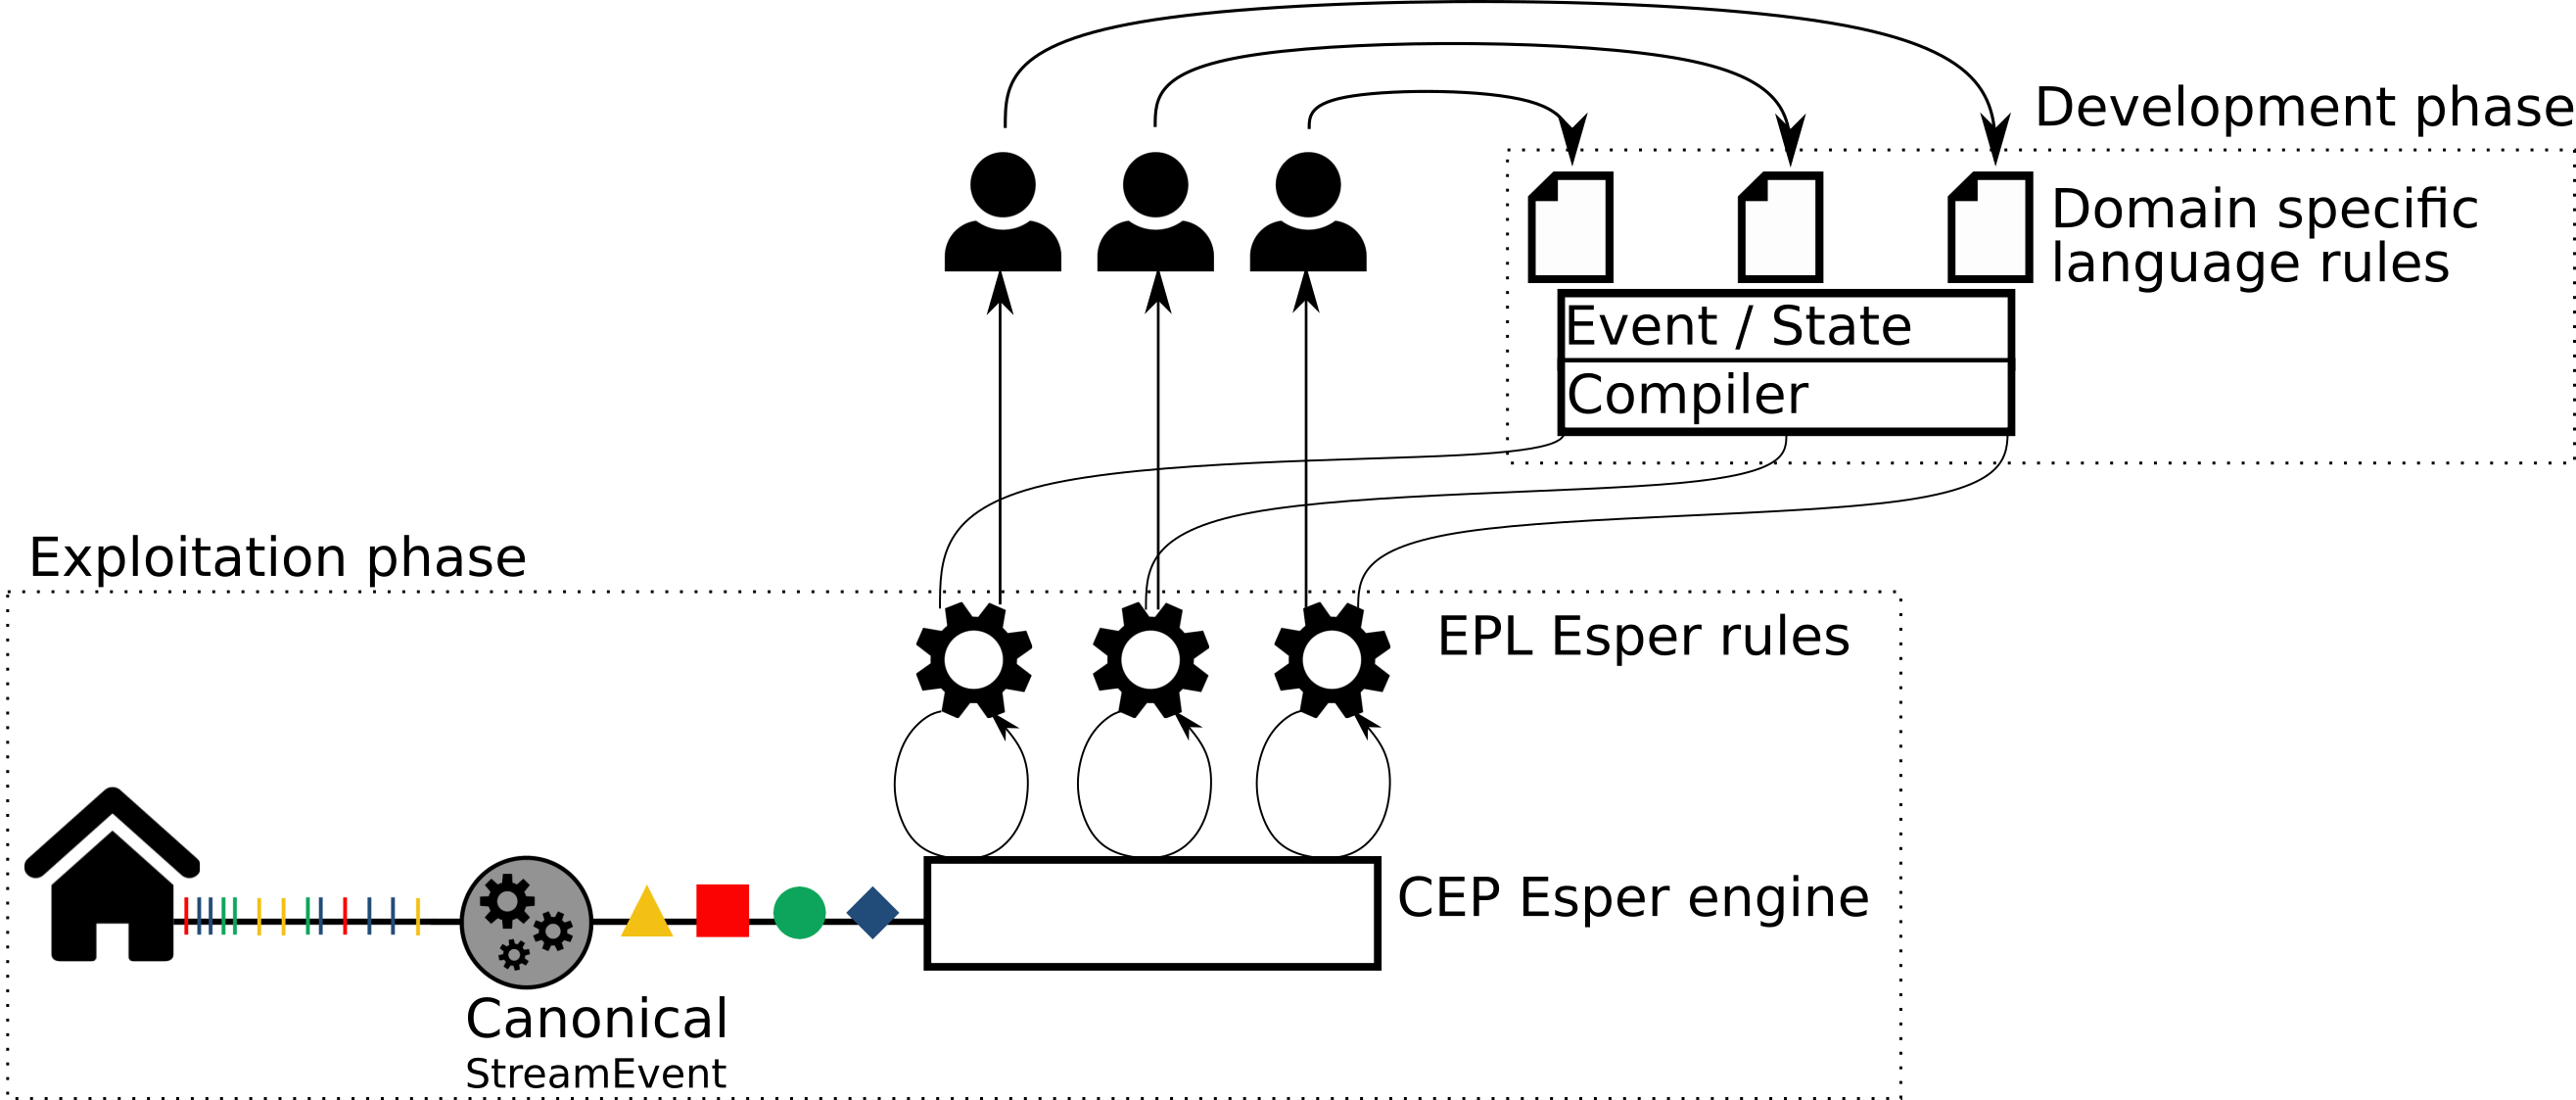
\includegraphics[scale=0.2]{gfx/approach}
\caption{Overall view of our domain-specific approach}
\label{fig:functionalarchi}
\end{figure}

\subsection*{Définition du service}
La première étape est initiée avec les intervenants qui expriment les scénarios de services, comme illustré plus tôt. Ces scénarios sont directement écrit dans notre langage dédié par l'intervenant, si ils ont le bagage nécessaire ou par un développeur de services en langage coeur.

\subsection*{Compilation du service}
Les services de haut niveau sont compilés dans des règles de plus bas niveau dans un langage de traitement d'évènement. Ces règles rendent explicite les concepts spécifiques au domaine, tels que les états qui sont compilés vers des combinaisons d'évènements et les opérations relatives.

\subsection*{Exécution du service}
Pour être déployées, les règles sont ajoutés à un moteur de traitement d'évènement complexe (CEP). Notre moteur d'exécution de règle est basé sur Esper, un CEP open-source développé par EsperTech\footnote{http://www.espertech.com/esper/}. Esper propose des interface Java et C\# pour développer des programmes événementiels. Nous avons choisis Esper parce qu'il s'agit d'un moteur CRP populaire utilisé à la fois dans l'industrie et dans la recherche. Esper fournie un langage spécifique et déclaratif pour le traitement d'évènement complexes, appelé EPL (pour Event Processing Language). EPL permet de décrire des motifs d'évènements à identifier dans un flux d'évènements temps réel, en utilisant des opérateurs pour ordonner les évènements, des contraintes temporelles, {\em etc.} Esper ne permet pas de manipuler le concept d'état; il permet uniquement de traiter des évènements et nécessite donc quelques manipulations pour gérer un état. Dans notre implémentation, nous utilisons Esper avec règles EPL, compilées depuis des règles écrites en langage Maloya, et un flux d'évènement issue de domiciles sensibles au contexte, formattés en une forme canonique.

\subsection*{Forme canonique}
La forme canonique de données produites par un domiciles sensibles au contexte permet de faire les traitement de façon uniforme, indépendemment de leur format hétérogène original. Dans notre implémetation, la forme canonique de données, appelée {\em StreamEvent}, est introduite comme couche d'abstraction sur le flux d'évènements de données. Dans cette représentation, chaque évènement est un 4-tuple du type d'évènements, sa localisation, sa valeur, et l'horodatage de son occurrence.

\section{Validation}\label{sec:validation}

Cette section présente la validation de notre approche sur la plate-forme DomAssist. L'expressivité de notre langage est validé en redéfinissant des services existant sur cette plate-forme. La justesse de notre compilateur est validée en comparant les résultats de l'exécution de nos règles compilées avec des services existants et déployés sur la plate-forme. Enfin, l'efficacité de notre langage est validé en mesurant certains les performances pertinentes pour le domaine de notre implémentation.

%\begin{landscape}
\begin{figure*}[h]
  \scriptsize
  \begin{tabular}{|l|p{7cm}|c|c|c|c|l|} 
    \hline
    \multirow{3}{*}{\textbf{Name}}&\multirow{3}{*}{\textbf{Description / DSL}}&\multicolumn{4}{|c|}{\textbf{Metrics}}&\multirow{3}{*}{\textbf{Stakeholders}}\\
    \cline{3-6}
                                  &                 &\multicolumn{2}{|c|}{\textbf{DSL}}&\multicolumn{2}{|c|}{\textbf{EPL}}&\\
                                  & & \# events & \# states & \# events & \# not &\\
    \hline
%**********************************************
    Presence & \cellcolor{gray!15}Detect if cupboard status changes while no presence in kitchen& \multirow{2}{*}{1}& \multirow{2}{*}{1} & \multirow{2}{*}{2}& \multirow{2}{*}{1} & Sensor\\ % \cline{2-2}
    dependency  & \begin{lstlisting}             
      Cupboard becomes open $\textbf{occurs}$ $\textbf{while}$ Presence(Kitchen) is false 
    \end{lstlisting} & & & && installer\\
    % &  & & && &\\
    % &  & & & &&\\
    \hline
%**********************************************
    Departure & \cellcolor{gray!15} Detect if entrance door is opened at least for 5 minutes during calendar night time & \multirow{4}{*}{1} & \multirow{4}{*}{1} & \multirow{4}{*}{2}& \multirow{4}{*}{2} & Occupational\\
                                 alert & \begin{lstlisting}  
                                    Door is open $\textbf{for}$ 5 minutes $\textbf{occurs}$ $\textbf{while}$ Night time
                                  \end{lstlisting} & & & &&  therapist \\ 
                                 &  & & & && Caregiver \\
    \hline
%**********************************************
    \multirow{2}{*}{Door alert} &\cellcolor{gray!15} Detect if entrance door is opened at least for 5 minutes during their is no presence in entrance& \multirow{4}{*}{0} & \multirow{4}{*}{2} & \multirow{4}{*}{4}& \multirow{4}{*}{6} &User \\
                                  & \begin{lstlisting}
                                    Door is open $\textbf{occurs}$ $\textbf{for}$ 5 min $\textbf{while}$ Presence(Entrance) is false
                                  \end{lstlisting} & &  && &  Caregiver \\
                                  &  & & && & \\
    \hline
%**********************************************
    Long &\cellcolor{gray!15} Detect if no movement in Bedroom since 24 hours & \multirow{3}{*}{0} &\multirow{3}{*}{1} & \multirow{3}{*}{1}& \multirow{3}{*}{1} & Occupational\\ %\cline{2-2}
    inactivity & \begin{lstlisting}
      Presence(Bedroom) is false $\textbf{for}$ 24 hours
    \end{lstlisting} & & & &&  therapist \\
                                  & & & & && Caregiver \\
    \hline
%**********************************************
    Fridge &\cellcolor{gray!15} Detect if fridge remains open at least 5 minutes &\multirow{2}{*}{0} &\multirow{2}{*}{1} & \multirow{2}{*}{1} & \multirow{2}{*}{1} & User\\% \cline{2-2}
    opened & \begin{lstlisting} 
      Fridge is open $\textbf{for}$ 5 minutes
    \end{lstlisting}& & & && Caregiver \\
    \hline
%********************************************** 
    \multirow{2}{*}{Breakfast} &\cellcolor{gray!15} Detect cupboard and coffeemaker opening (any order) during breakfast period & \multirow{3}{*}{2} & \multirow{3}{*}{1}&\multirow{3}{*}{3}&\multirow{3}{*}{1} & User\\% \cline{2-2}
                                  &  \begin{lstlisting} 
                                    $\textbf{\{}$Cupboard becomes open $\textbf{and}$ CoffeeMaker becomes on$\textbf{\}}$ 
                                    $\textbf{occurs}$ $\textbf{while}$ BreakfastTime 
                                  \end{lstlisting} & & & && Caregiver \\
    \hline
%**********************************************
    Lunch &\cellcolor{gray!15} Detect freezer opening and stove use in the 10 minutes following or freezer opening during stove use & \multirow{8}{*}{3} & \multirow{8}{*}{2} & \multirow{8}{*}{5}& \multirow{8}{*}{3} & Caregiver \\ %\cline{2-2}
    reheat &\cellcolor{gray!15} all during lunch period & & & & & User \\ %\cline{2-2}
     & \begin{lstlisting}  
      $\textbf{\{}$ ( Freezer becomes open $\textbf{precedes}$ $\textbf{within}$ 10 minutes 
          Stove becomes on ) 
        $\textbf{or}$ 
        ( Freezer becomes open $\textbf{occurs}$ $\textbf{while}$ 
          Stove is on ) $\textbf{\}}$
      $\textbf{occurs}$ $\textbf{while}$ Lunch Time
    \end{lstlisting}& & & & & \\                              
    \hline
%**********************************************
    \multirow{2}{*}{Dinner} & \cellcolor{gray!15} Detect fridge opening and microwave use (any order) during dinner period & \multirow{3}{*}{2} & \multirow{3}{*}{1} &\multirow{3}{*}{2} & \multirow{3}{*}{1} & User\\ %\cline{2-2}
                                  & \begin{lstlisting}  
                                    $\textbf{\{}$Fridge becomes open $\textbf{and}$ Microwave becomes on$\textbf{\}}$
                                    $\textbf{occurs}$ $\textbf{while}$ Dinner Time
                                   \end{lstlisting} & & & && Caregiver \\
    \hline
%**********************************************
    Go &\cellcolor{gray!15} Detect end of presence in bathroom and begin of presence in bedroom in the 10 minutes following & \multirow{5}{*}{2} & \multirow{5}{*}{1} & \multirow{5}{*}{3} & \multirow{5}{*}{2} &Caregiver \\ % \cline{2-2}
    to bed  &\cellcolor{gray!15} during go-to-bed period & & & & &User \\ 
    &  \begin{lstlisting} 
      ( Presence(Bathroom) becomes false $\textbf{precedes}$ $\textbf{within}$ 10 minutes 
        Presence(Bedroom) becomes true ) 
      $\textbf{occurs}$ $\textbf{while}$ Go-to-bed Time
    \end{lstlisting} & & & && \\
    \hline
%**********************************************
    \multirow{2}{*}{Wake-up} &\cellcolor{gray!15} Detect end of presence in bedroom and begin of presence in kitchen in the 10 minutes following & \multirow{5}{*}{2} & \multirow{5}{*}{1} & \multirow{5}{*}{3} & \multirow{5}{*}{2} & Caregiver \\ %\cline{2-2}
                                  &\cellcolor{gray!15} during go-to-bed period & & & & &User \\ 
                                  & \begin{lstlisting} 
                                    ( Presence(Bedroom) becomes false $\textbf{precedes}$ $\textbf{within}$ 10 minutes
                                      Presence(Kitchen) becomes true )
                                    $\textbf{occurs}$ $\textbf{while}$ Wake-up Time
                                  \end{lstlisting}& & & && \\
                                  % &  precedes within 10 min& & & && User\\
                                  % &  Presence(Kitchen) becomes true ) & & & && \\
                                  % &  occurs while Wake-up-time & & & && \\
    \hline
%**********************************************
    Commfailure &\cellcolor{gray!15} Detect any sensor that fails to communicate & \multirow{2}{*}{1} & \multirow{2}{*}{0} & \multirow{2}{*}{1} & \multirow{2}{*}{0} & Platform \\% \cline{2-2}
      warning& \begin{lstlisting}  
        Commfailure( Any ) becomes true 
        \end{lstlisting}& & & && maintainer \\
    \hline
%**********************************************
    Commfailure &\cellcolor{gray!15} Detect any sensor that has failed to communicate since 24 hours & \multirow{4}{*}{0} & \multirow{4}{*}{1} & \multirow{4}{*}{1} & \multirow{4}{*}{1} & Platform\\ %\cline{2-2}
      alert&  \begin{lstlisting} 
        Commfailure( Any ) is true $\textbf{for}$ 24 hours 
        \end{lstlisting}& & & &&  maintainer \\
                                  & & & & && Sensor \\
                                  & & & & && installer \\
    \hline
%**********************************************
    Battery & \cellcolor{gray!15} Detect battery level of any senser that become less than 5\% & \multirow{2}{*}{1} & \multirow{2}{*}{0} & \multirow{2}{*}{1} & \multirow{2}{*}{0} & Sensor\\ %\cline{2-2}
    alert & \begin{lstlisting}
      BatteryLevel( Any ) becomes $\textit{less than}$ 5 
      \end{lstlisting}& & & && installer\\
    \hline
  \end{tabular}
  \caption{Services examples}
  \label{app_examples}
\end{figure*}
%\end{landscape}

\subsection{Expressivité}\label{validation:expressiveness}
Pour validé l'expressivité de notre langage, nous avons réimplanté 55 services déjà déployés dans DomAssist. Ces services sont les variation des 13 familles de règles listés en Figure~\ref{app_examples}. Des variations sont requises pour satisfaire les spécificités des personnes âgées. Par exemples, la détection des activités du quotidien comme la préparation du repas et le lever/coucher, doit être personnalisée pour chaque utilisateur dans le respect des capacités de mesures des interactions l'environnement, périodes de reconnaissance des activités, et des périodes de temps entre les séquences d'intéractions. Par exemple, pour préparer le petit déjeuner, une personne âgée peut utiliser un presse agrume électrique et prendre un verre dans un placard spécifique, alors qu'un autre peut utiliser une bouilloire et ouvrir le frigidaire our prendre du lait.

Réécrire une éventail de service nous permet de valider que notre langage et ses concepts sous-jacents (évènements, états, opérateurs d'Allen) sont suffisamment expressif pour couvrir des cas réels de services dans le domaine du maintien à domicile de personnes âgées.

%\subsection{Compilation}\label{validation:compilation}
\subsection{Exactitude}\label{validation:results}
%We did not attempt to prove the correctness of our DSL compiler with respect to a formal semantics of its operators, although this work would be of interest. Instead, we empirically validated the correctness of the compiled services by a combination of visual code inspection and extensive testing. We performed manual inspection of all the intermediate forms described earlier (core DSL, EPL pseudo-code, Esper EPL) to ensure that they remain consistent with their original counterparts.

Nous avons validé empiriquement l'exactitude de nos services compilé par des inspections visuels et des tests étendu. Nous avons inspecté manuellement les formes intermédiaires décrites précédemment (pseudo-code EPL, EPL Esper) pour nous assurer de la cohérence des résultats des différentes étapes de compilation.

Ensuite, nous avons validé la sortie du compilateur ({\em i.e.,} règle EPL résultante) en deux phases. Premièrement, nous avons testé les règles en les exécutant sur des fichiers de logs provenant du projet DomAssist. Ces logs contiennent des évènements horodatés produits par tous les capteurs de l'infrastructure, qu'ils soient matériels ou logiciels. Les résultats ont été automatiquement vérifié par des scripts Perl, implantant les même spécifications de service. Ces scripts sont plus simple à écrire que les vrais applications puisqu'ils exécutent les logs de données, ils n'ont ainsi pas à traiter les résultats en temps réel, et n'ont pas à traiter avec l'infrastructure de capteurs.

%We repeatedly compared the results produced by the compiled DSL services and the scripted specifications on extended log histories. This iterative process allowed us to refine our compilation schemas until it produced the same results as the scripted specifications.

Dans une seconde phase, nous avons connecté nos services au flux d'évènements temps réel sur la plate-forme de production pour neuf utilisateurs pendant un mois, en parallèle des services existants écrits en Java. Aucune différences n'ont été observées dans les résultats entre les deux systèmes (Java et règles compilées depuis notre langage). De plus cette phase nous à permis d'évaluer les performances à l'exécution de notre approche.


\subsection{Performances}\label{validation:performance}
Pour valider l'utilisabilité de notre approche à base de langage dédié en pratique, nous avons mesuré en conditions réelles, les performances des règles EPL produites par notre compilateur avec deux indicateurs: la latence de détection, et la consommation mémoire de notre moteur d'exécution. Les règles sont exécutées sur notre serveur de production (quad-core Intel(R) Xeon(R) E5-2407 v2 2.4 GHz CPU et 125GB RAM).

La latence de détection d'une règle donne le temps entre le dernier évènement qui déclenche une règle, et sont déclanchement effectif. Une latence faible indique que la règle est suffisamment réactive pour un usage pratique. D'après nos mesures, cette latence pour nos règles est toujours inférieur à une seconde. Cet ordre de grandeur est parfaitement compatible avec le type de règle qui sont implanté dans la plate-forme pour le maintien à domicile des personnes âgées.

Nous avons également mesuré la consommation mémoire de notre implémentation pour nous assurer qu'elle peut passer à l'échelle pour des centaines d'utilisateurs et des dizaines de services. D'après nos mesures, la consommation mémoire est de 352MB en moyenne pour 55 règles, traitant les données de 129 domiciles pendant un mois 24 heures sur 24. Encouragés par ces résultats, nous avons entrepris d'explorer la possibilité d'appliquer notre approche et notre implantation sur une architecture plus limitée, mais plus accessible et fréquemment utilisée en informatique ubiquitaire, un Raspberry Pi 3 (quad-core ARM Cortex-A53 1.2 GHz CPU et 1GB RAM). Durant cette expérimentation, nous avons exécuté les même 55 règles avec les mêmes 129 installations pendant un mois. La consommation mémoire constatée est de 173MB en moyenne. Cette moindre consommation mémoire sur le Raspberry Pi s'explique par son architecture 32-bit.
Ces mesures nous montre que notre apporche est applicable tant sur une infrastructure cloud que sur une infrastructure embarquée directement à l'intérieur du domicile.

\section{Discussion}

Our DSL bridges the gap between high-level domain concepts and low-level mechanisms of event handling. As a consequence, it contributes to making rules more concise and  to simplify their development, by encapsulating details of event handling in a compiler.  Indeed, the original Java applications implementing HomeAssist services contain manually implemented timed automata, which recognize the sequences of events corresponding to each DSL rule.  Timing constraints are explicitly handled by using a timer service, producing timeout events that are inserted in the stream of events, produced by the sensor infrastructure.  In our DSL rules, these low-level details of state and time handling are included in the semantics of operators.  For instance, the role of explicit timers corresponds the parameters of our time-constrained operator variants. This lowers the efforts to write rules and to make them more predictable.

\subsection*{Limitations}

Our approach is a first step towards simplifying the development of context-aware applications in the domain of aging in place, and presents a number of limitations.

First of all, our DSL only is dedicated to recognizing contexts. It provides no constructs for performing actions on the environment. These must be currently programmed in a generic programming language. It would be useful to extend our domain analysis to also cover the control part of typical applications, and to derive domain-specific concepts and notations to perform actions.

As far as applications are concerned, we have designed and tested our DSL only on services in the domain of aging in place, which involves a specific set of composition operators. However, our DSL can express rich, arbitrarily nested combinations. It would be interesting to apply it to other domains of context-aware applications in the future.

Finally, our rules always return boolean values. However, context-aware information may sometimes be more general than strictly binary. For instance, a daily activity such as meal preparation might be detected in a more nuanced way as a probability between 0 and 1, to cope with some amount of deviations from the user's routine. Currently, in our DSL the different routine variations must be coded as different rules, which is not always practical. In the future, it would be interesting to consider extending our approach with operators returning non-boolean values.
% Such fuzzy detectors are sometimes used in the domain of aging in place.

\section{Conclusion}
%**********************************************
%**********************************************

We have proposed a new approach for developing context-aware services in a smart home, by
analyzing a range of existing data processing layers in the domain of aging in place. We have identified key concepts and operations specific to context-aware processing. Based on this analysis, we have introduced a context-aware, domain-specific language and its software architecture, which allow to put in synergy the stakeholders of a context-aware home by providing them with a unified approach to designing and developing services. Our approach offers context aware-specific abstractions and notations, within a data-centric and data-driven paradigm.

We have validated our approach by applying it to an assisted living platform for aging in place. In particular, we have used our domain-specific language to re-implement existing services of the assisted living platform. These services were deployed and successfully tested for their effectiveness in performing the specific tasks of the stakeholders: detection of daily activities, detection of user risks, sensor failure, {\em etc.}

\chapter{Compilateur}
\begin{preamble}

\end{preamble}

\section{Opérateurs}
\section{Compilation vers pseudo-code EPL}

\section{Compilation vers EPL}
\chapter{Conclusion}
\section{Discussion}
\section{Perspectives}
%langage visuel
%configuration par la simulation
%\input{test}
% %Partie Théorique
% \input{TSA}
% \input{priseencharge}
% \input{technologies}


\bibliography{sample}

\end{document}
